\documentclass[11pt]{sdm}
\usepackage{xcolor}
\usepackage{float}
\usepackage[utf8]{inputenc} 
\usepackage{indentfirst}
\usepackage{listings}
\usepackage{hyphsubst}
\usepackage{amsmath}
\usepackage{enumitem}

				  
\lstdefinestyle{customc}{
  belowcaptionskip=1\baselineskip,
  breaklines=true,
  frame=L,
  xleftmargin=\parindent,
  language=C,
  showstringspaces=false,
  keywordstyle=\bfseries\color{green!40!black},
  commentstyle=\itshape\color{purple!40!black},
  identifierstyle=\color{blue},
  stringstyle=\color{orange},
}

\lstset{escapechar=@,style=customc,numbers=left,literate={~} {$\sim$}{1}}


%Number the pages
\pagestyle{plain}

\title{Software Fault Isolation using the CompCert compiler}
\author{Alexandre \textsc{Dang}}
\supervisorOne{Frédéric \textsc{Besson}}
\team{Team CELTIQUE}

\school{supelec}

\domain{Domaine: Cryptography and Security}

%write your abstract here
\abstract{
Software Fault Isolation (SFI) is a software method which allows one to isolate the execution of possibly dangerous modules, hence preventing any risks of corruption of our system due to these modules. Even though SFI has multiple benefits it still has troubles dealing with Returned Oriented Programing attacks which aims at diverting the control flow through the return addresses. During our internship we implemented a flexible solution against these attacks with the certified compiler CompCert. Our approach transforms the stack layout in order to easily know the locations of the return addresses enabling us to protect them from being overwritten illegally. 
We made an implementation with CompCert which is almost complete that successfully blocks buffer overflows. 
In return we have a diminution of the efficiency depending of the number of runtime checks added. However multiple ideas exist to reduce this overhead like having a finer detection of dangerous instructions with the use of static analysis.
}
\setcounter{tocdepth}{2}
\begin{document}
\maketitle

%*****************************************************************%

\newpage
\section{Introduction}
IT projects regularly need to use external modules in their programs. However these modules can come from unknown sources and we don't have any guarantees that they don't contain any bugs or malicious code. Software Fault Isolation is an approach which wants to face this issue by verifying certain security properties during the execution of the dangerous modules.

A rising interest for the techniques of Software Fault Isolation (SFI) has appeared in the field of cyber security. SFI is a mean to protect the memory of a program with software solutions. 
The idea is that a protected program can load in its own memory space dangerous modules without them being able to compromise its execution.
To make it happen, SFI isolates the dangerous modules in reserved areas of the memory called sandboxes. This operation is realised by a code generator that modifies the code of the dangerous modules in order to have them comply with the security properties defined by SFI. 
Afterwards the modified code of the modules will go though a verifier that will check that the modifications introduced before are present and valid.

SFI techniques are applicable in multiple fields. An implementation has already been made for Google Chrome~\cite{Yee:2010:NCS:1629175.1629203}\cite{Sehr:2010:ASF:1929820.1929822} called NativeClient. We can also imagine using SFI for critical systems that have to execute external modules.
For example computer clusters or system kernels could require the use of SFI to safely execute external modules.

SFI has multiple strong points which explains its current appeal. Firstly, we can note high performances due to the execution of the modules natively in the address space of the protected program. This trait is quite important since the most popular memory protection mechanisms nowadays use hardware solutions and suffer from great overheads. Another benefit of SFI is that it requires a relatively small \textit{Trusted Computing Base} (TCB). Indeed only the verifier needs to be in the TCB and not the code generator. Having a small TCB means that only a minor portion of the code (the verifier) needs to be trusted to have a correct implementation of SFI.

However SFI has still difficulties to deal with the protection of the \texttt{ret} instruction that uses return addresses on the stack. A big part of modern attacks like \textit{Return Oriented Programming} attacks focus on deviating the control flow through return addresses. Therefore it is absolutely necessary to have a good protection for return addresses. The SFI solutions found in the literature are not easily adaptable or bring a lot of overhead to the compiled modules. \\
Hence we propose a solution which is more flexible and faster to address this specific issue of SFI.
The idea is to modify the stack structure to have an easy way to figure out the return addresses locations in the stack.
We set the frames size to a constant value in order to have the return addresses separated by a fix offset. Afterwards we modify the dangerous code by adding runtime checks  which take advantages of the new stack layout to prevent any instruction to overwrite the return addresses. 

This internship report will firstly present Software Fault Isolation, its principles, the existing implementations and especially a version using CompCert the certified compiler. CompCert will also be the compiler we chose to implement our solution to defend programs against ROP attacks. We will then present an overview of our approach with fixed frames size with a discussion of our idea. Afterwards we will explain in details the implementation we made of our approach with CompCert during the span of the internship. To conclude we will evaluate the different results obtained with our implementation and propose ideas to improve our solution in the future.



\newpage
\section{Software Fault Isolation}
\label{sec:sfi}

	We introduce here \textit{Software Fault Isolation} (SFI) which inspired us the idea to protect return addresses through fixed stack frame size. SFI aims to protect a main program from the different modules that it will need to use. These modules will be loaded in the same memory space as the main program but in a confined area called \textit{sandbox}. The SFI mechanism is composed of two elements: a code generator and a verifier. The generator transforms the assembly code of the hazardous modules so that they will be constrained in the sandbox. The verifier operates just before loading the modules in the memory. It checks the if SFI transformations introduced by the generator are still present and valid. For the rest of the document we will reserve the word ''program'' to refer to the code protected by SFI and ''module'' to refer to the hazardous code.

\subsection{Principle}

The main principle behind SFI was first presented in the work of Wahbe and al.~\cite{Wahbe:1993:ESF:173668.168635}.
Later works that will be introduced Chapter~\ref{sub:sfi_other} are all based on the foundations of SFI detailed here.
The implementation described here was realised for a RISC architecture like MIPS or \textit{Alpha}.

SFI considers that a malicious code is effectively contained in the sandbox if these three security properties hold true:
\begin{itemize}
	\item \textbf{Verified code}, only instructions that have been checked by the verifier will be executed 
	\item \textbf{Memory safety}, malicious modules will not do any \textit{write} or \textit{jump} operations out of the sandbox
	\item \textbf{Flow control integrity}, every flow control transfer from hazardous modules to the main program is identified and verified
\end{itemize}
The first property protects us against self-modifying code which could bypass the SFI measures. \textit{Memory safety} prevents any illegal access to the memory of the protected program. The last property allows us to authorized only licit interactions between the program and its modules. SFI forbids any call from malicious modules that could modify the flow control of the program. If the flow control was fiddled with, it could lead to an unexpected behaviour of the program which we want to avoid.

The code generator transforms the assembly code of the hazardous modules so that they respect the security properties presented before. The generator is integrated to the compiler which will create a \textit{sandboxed executable}. Afterwards this executable will be checked by the verifier before being loaded into the memory. 
The verifier checks that the transformations introduced by the generator are present and valid. 
If the verification fails the module will be rejected and will not be executed. We can note that we only need to trust the verifier to prevent running any dangerous module. 
It is one advantage of SFI, only the verifier needs to be in the \textit{Trusted Computing base} (TCB).


\subsubsection{Code generator}
\label{ssub:Code generator}
To protect the program from its modules, the generator will restrain every write and jump instructions of the modules to addresses of their sandbox.
The generator has to face three issues to do so. The first one is to introduce protection mechanisms before every dangerous instructions. For example, assessing that the destination address of a jump instruction is an authorized one.
Secondly, we have to make sure that these protection mechanisms can't be avoided. 
Finally, the transformations introduced have to only authorized legal calls from the sandbox to the protected program by using entry points specified by the latter. For example, Google Chrome only allows its modules to use a specific interface to interact with the browser. This way the modules can't disrupt the flow control of Google Chrome easily.
\paragraph{Confining memory accesses.}
\label{par:Confining memory accesses}
The main program memory should avoid being corrupted by its modules. SFI aims to isolate these modules in a reserved area of the program memory called sandbox.
The sandbox is a contiguous memory area which size is a power of two. These requirements ease the confinement of the modules in their sandbox by allowing the use of bit arithmetic which accelerates the process.
In fact two sandbox are allocated, the first one for the code segment and the second for the data segment. In these conditions we only need to verify that the most significant bits of the targeted address match those of the sandbox. For example, if we allocate to the sandbox the memory \texttt{[0xda000000~-~0xdaffffff]}, then all the addresses which most significant bits match \texttt{0xda} are located in the sandbox. Thus all the SFI transformations will restrain the memory writes and jumps to the addresses of the sandbox area. In our example, we will limit ourselves to the addresses whose most significant bits are \texttt{0xda}, this sequence of bits is also called \textbf{tag}. Each tag are specific to an unique sandbox and this designation will be used repeatedly in our report. 

During the code generation phase every direct memory addressing will be easily detected with static analysis. 
The transformation will be simple, the targeted addresses will simply have their most significant bits replaced by the tag of the sandbox. Another possible reaction is to reject the code if it is explicitly unsafe. The real issue appears when faced with a write or a jump using indirect memory addressing. Indeed in these cases the destination address is stored in a register and we can't access this value during the compilation. However to address this situation SFI injects in the code of the dangerous module runtime checks that are called \textit{sandboxing}.

\begin{figure}[!ht]
\centering
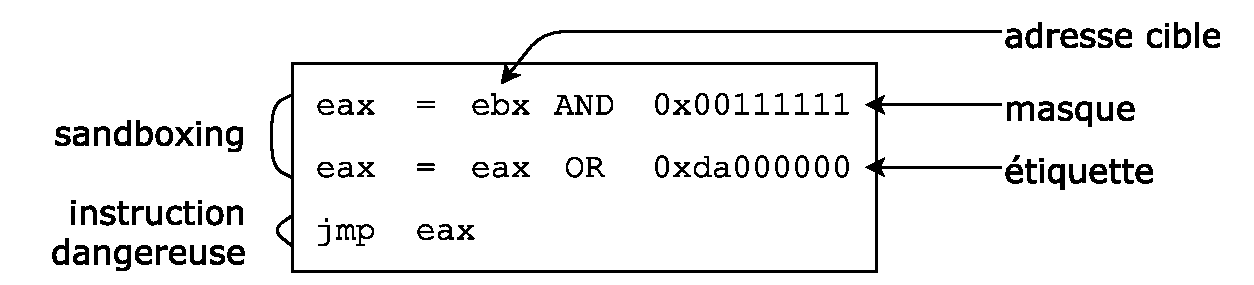
\includegraphics[scale=0.5]{images/algo_sandboxing.pdf}
\caption{Pseudo code of the sandboxing operation}
\label{algo_sandbox}
\end{figure}


Figure~\ref{algo_sandbox} represents an example of the sandboxing operation. The sandboxing starts with a masking operation which sets the most significant bits of the address stored in the register \texttt{ebx} to zero. Afterwards the second instruction write the tag of the sandbox on the bits it just reinitialised before. Hence we are sure that the \texttt{jmp} instruction will target a location in the sandbox of the dangerous module. We can note that the sandboxing does not change the behaviour of the module if the targeted address was already in the sandbox. This principle is called \textit{transparency}, SFI transformations does not change the execution of safe programs. For the write instructions the principle is the same. We will inject the sandboxing instructions before every write in the memory using an address stored in a register.

\paragraph{Protection of sandboxing mechanisms.}
\label{par:Protection of sandboxing mechanisms}
We made sure in the previous section that any dangerous modules can't either jump or write on a location out of its sandbox. Now we also want to protect the sandboxing operations to prevent any malicious code to bypass the runtime checks inserted by SFI. Using the example Figure~\ref{algo_sandbox}, we could imagine code which directly jumps on the \texttt{jmp eax} instruction. To protect the sandboxing, the solution is to establish dedicated registers exclusively used for sandboxing. These registers won't be available anymore for the rest of the code. Sandboxing requires three dedicated registers for each sandbox. First register will be used to keep the mask value (\texttt{0x00111111} in Figure~\ref{algo_sandbox}). Second register is reserved to store the tag of the concerned sandbox (\texttt{0xda000000} in Figure~\ref{algo_sandbox}). And the third dedicated register is used to manage the operations contained in the sandboxing, in our example Figure~\ref{algo_sandbox} it would be the register \texttt{eax}. This way during the whole execution of the dangerous module \texttt{eax} will only store addresses of its sandbox. Then even if malicious code can jump directly to the instruction \texttt{jmp eax} we will still be sure that we will stay in the sandbox. 
Worst case scenario the value stored in \texttt{eax} was wrong and the dangerous module crash or has unexpected behaviour. As long as the protected program is not affected the protection is considered successful.
These dedicated registers are never used by the rest of the code and their values can't change except during sandboxing operations.

Since we have two sandboxes, one for the data and one for the code we then have a total of six dedicated registers. However SFI manages to reduce the number of dedicated registers to five by using a common mask value for both the sandbox.

We can question ourselves on the efficiency of SFI when we remove five registers for the execution of the normal code. However, in the modern RISC architecture like MIPS or Alpha there are generally 32 registers. Moreover the experiments~\cite{Wahbe:1993:ESF:173668.168635} show that removing five registers for the gcc compiler impacted insignificantly the efficiency of the programs tested.

\paragraph{Controlled interactions with the protected program.}
\label{par:Controled interactions with the protected program}

	It is necessary for SFI to also control the different interactions that dangerous modules have with the main program. Without restrictions, malicious modules could, for example, make function calls with wrong parameters which could compromise the state of the main program. 
To avoid such situation, SFI needs the main program to define an interface which describes all the authorized entry points available to external modules. This interface also includes the range of authorized values for the different parameters. 
For example Google Chrome has created an API which can be called by the different modules to access the resources of the browser.
SFI will then transform the modules so that every interaction with the main program will be done through connectors called \textit{stubs}. These stubs are part of the Trusted Computing Base (TCB) of SFI. In relation with the interface of the main program, the stubs make sure that function calls from the dangerous module to the main program are licit. If they are not, the stubs will reject the function calls. 
System calls are controlled the same way, the stubs will first check the call and if it is authorized it will transmit the system call to the main program. Then the main program will execute the system call to the kernel and return the results to the module.

\subsubsection{Code verifier}
\label{ssub:Code verifier}
The verifier is the last element of the SFI chain. Consequently it is necessary for it to be part of the TCB contrary to the code generator. Even if the code generator is flawed the verifier will reject every executable which does not comply with the SFI requirements. Nevertheless the verifier relies on the generator work to do the checking. The verifier analysis just asserts that the SFI transformations made by the generator are present and valid. Therefore it's not possible for a binary which does not go through the generator to be validated by the verifier even if the binary is safe.

The first step of the verification is to disassemble the given binary. The implementation of Wahbe et al.~\cite{Wahbe:1993:ESF:173668.168635} was made for the architectures MIPS and Alpha. In these architectures all the instructions are 32 bits long. This particularity makes the disassembly easier since we just need to treat sequences of 32 bits. The second step is to check that the SFI transformations are present and valid. The first condition is that the registers dedicated to store the mask and the tags should never be modified. Afterwards we need to check that the sandboxing operations are done correctly. For that we define in the modules some sandboxing areas. These areas begin every time that one of the dedicated registers is modified. Then these sandboxing areas are closed when we do a jump or a write with a dedicated register or when there are no instructions left. To validate a sandboxing area we verify that the dedicated register used for the jump or the write will have an authorized value at then end of the area. In other words the dedicated register will have a value whose most significant bits are equal to the tag of the sandbox.

\subsubsection{Pros and cons}
\label{ssub:Pros and cons}

SFI aims to isolate the execution of dangerous modules in a designated area of the protected program memory. For this, SFI is composed of a code generator tasked with producing a sandboxed binary and a verifier which checks if the executable complies with the SFI properties.
It is imperative that the verifier is part of the TCB in order to have SFI only accept safe code. We can note that to be functional SFI does not need an extensive TCB, only the verifier needs to be part of it. Another advantage is that SFI is not language dependant, the approach does not depend of the source language of the code. In return SFI is architecture dependant, the transformations will not be the same on x86 or on MIPS. Another con is that the sandboxed code is also less efficient and also bigger. Nevertheless only the dangerous modules are sandboxed which usually represents a minor part compared to the whole execution. A last inconvenient is that the presented implementation only includes MIPS and Alpha architecture but later works adapt SFI to other architectures.

\subsection{SFI for other architectures}
\label{sub:sfi_other}
In the work of Wahbe et al.~\cite{Wahbe:1993:ESF:173668.168635} the methods used was made for the RISC architecture and especially MIPS and Alpha. We detail in this section the necessary modifications created to adapt SFI to x86 and ARM.

\subsubsection{SFI for CISC architectures}
\label{ssub:SFI for CISC architectures}
	Contrary to RISC architecture in a CISC architecture the instructions may have different lengths. This particularity introduces two issues for SFI. First of all it is possible for an instruction to jump in the middle of another instruction which would totally change the flow of the program. Moreover the disassembly phase of the verifier becomes much more complex and the assembly obtained is not always reliable.
In RISC architecture there is a natural alignment since all the instructions are 32 bits long. The processor then always makes sure that it jumps on an address respecting the 32 bits alignment. This way the code is protected from this kind of threats. In CISC it becomes a serious issue which can't be ignored by SFI.

To face this problem, Pittsfield~\cite{Mccamant_evaluatingsfi} proposes to create an artificial alignment using chunks of memory of constant size. To have this approach work the sandboxed code needs to verify some additional properties:
\begin{enumerate}
	\item The sandbox is divided by chunks of constant length equal to a power of two
	\item Every instruction targeted by a jump has to be located at the beginning of a chunk
	\item Every function call has to be located at the end of a chunk
	\item It is forbidden for an instruction to overflow on multiple chunks
	\item Every chunk which are not full are filled with \texttt{no-op} instructions
\end{enumerate}

The first rule allows us to create an artificial alignment on the chunks length. The rule number 2 enforces the property that every destination of a jump instruction will be aligned. In other words with memory chunks of sixteen bits, every jump will have its target address with the four least significant bits equal to zero. 
The rule~3 guarantees us that every return address from a function call will be the beginning of a chunk and then will be aligned. The rule number 4 is necessary for the instructions to respect the artificial alignment. \\
From all these rules we can deduce an atomicity property for the memory chunks. More explicitly, since it is not possible to jump in the middle of a chunk we can be certain that all the instructions of a memory chunk will be executed atomically.
This atomicity property is a big gain for SFI because it allows us free ourselves from the use of dedicated registers to SFI. Indeed these dedicated registers were used in order to prevent bypassing the sandboxing of dangerous write or jump. By using the artificial alignment we can make sure that it is not possible to avoid the sandboxing operation and execute the dangerous instruction directly.
We just need to gather all the sandboxing operations with their dangerous instruction in the same memory chunk, the atomicity of the chunks will then protect our mechanism.

The downside of this approach is that the artificial alignment slows down the execution of the modules concerned. Benchmarks carried out show a diminution of the average performances by 21\% compared to a non-modified module.

\subsubsection{NativeClient the implementation of SFI by Google}
\label{ssub:NativeClient the implementation of SFI by Google}
Google developed NativeClient~\cite{Yee:2010:NCS:1629175.1629203} which is included by default on its browser Google Chrome. Chrome uses SFI to execute possibly dangerous modules. These modules are executed natively and show better performances than with JavaScript. NativeClient is certainly the most complete implementation of SFI nowadays.

\paragraph{NativeClient for x86-32.}
\label{par:NaCl_32}

The first version of NaCl (Native Client) was developed for the architecture x86-32~\cite{Yee:2010:NCS:1629175.1629203}. This implementation combines the usage of x86 memory segments with ideas of the previous approach for CISC architecture. In order to make NaCl complies with the security properties of SFI, Google created multiple rules presented Figure~\ref{nacl_constraints}.

\begin{figure}[!ht]
\centering
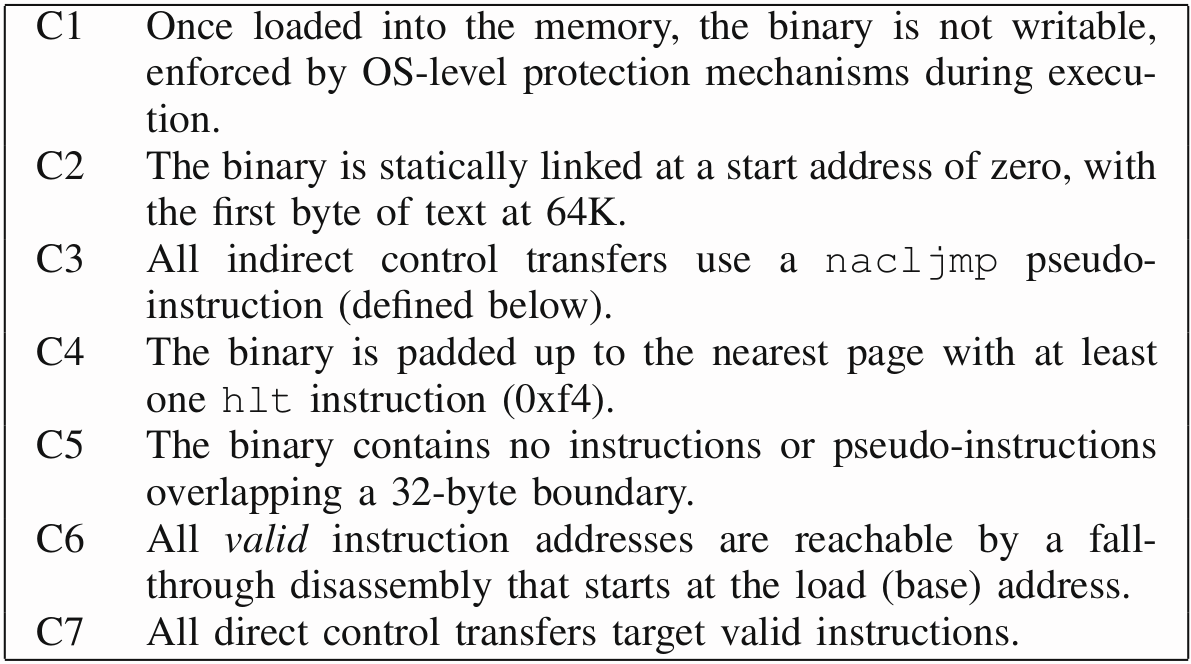
\includegraphics[scale=0.25]{images/nacl_constraints.png}
\caption{NaCl rules (Bennet Yee et al.~\cite{Yee:2010:NCS:1629175.1629203}, Table~1)}
\label{nacl_constraints}
\end{figure}


NaCl uses x86 memory segments to confine the data memory area in continuous memory area. These memory segments are then used as natural sandbox for the writing instructions. Therefore we don't need to do sandboxing operations for write instructions since it is handled natively by the processor.

Afterwards we still need to confine the jump instructions to the sandbox. NaCl uses the memory segment \texttt{CS} which is a code segment. We force the segment to start at the address 0 like indicated by the rule C2 of Figure~\ref{nacl_constraints}. This way the most significant bits of the addresses in the sandbox are equal to 0 and we can then reduce the sandboxing to two operations instead of three like presented Figure~\ref{nacl_jump}.
Moreover NaCl guarantees us that the destination address is a multiple of 32 (rule C5 of Figure~\ref{nacl_jump}). This technique is inspired from the approach using memory chunks seen earlier. This operation  is called \texttt{nacljmp} by NaCl (rule C3 of Figure~\ref{nacl_jump}).

\begin{figure}[!ht]
\centering
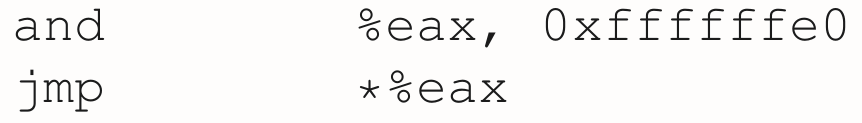
\includegraphics[scale=0.22]{images/nacl_jump.png}
\caption{\texttt{nacljmp} the reduced sandboxing operation (Bennet Yee et al.~\cite{Yee:2010:NCS:1629175.1629203})}
\label{nacl_jump}
\end{figure}

We can see that the rules C1 and C6 of Figure~\ref{nacl_jump} guarantee us that the disassembly of the binary is reliable. C1 in particular allows NaCl to protect against auto modifying code. If those were accepted they would render SFI pointless. This way with a reliable disassembly NaCl can make sure that only the analysed instructions can be later executed. This core property to SFI is rarely evoked in the other works and NaCl is the only one which implements it explicitly.

NaCl also choses to forbid system calls, instructions that modify the memory segments state and replace the \texttt{ret} instruction with a \texttt{pop} and a \texttt{nacljmp} to the return addresses.
This last measure was taken to control the inherent vulnerability of \texttt{ret} instruction. \texttt{ret} uses an address stored in the stack as its destination address. Since the return addresses are read from the stack they are subject to concurrency from the different threads. Therefore even if we add a runtime check on the values of return addresses we do not have the guarantee that the value has not changed between the sandboxing and the execution time of \texttt{ret} (Time Of Check Time Of Use).

\paragraph{NativeClient for X86-64 and ARM.}
\label{par:NativeClient for X86-64 and ARM.}
NaCl aims to be used with the popular browser Google Chrome, so Google needs to adapt its product to the most used architecture which are x86-64 and ARM (smartphones). These two versions of NaCl are evolutions from the x86-32 version modified to fit x86-64 and ARM specificities. For example, these two architectures do not have memory segments and NaCl was forced to reuse more classical methods of sandboxing for the write instructions. These implementations do not bring many novelties to SFI, hence we will not detail the work done but more information can be found on their publications~\cite{Sehr:2010:ASF:1929820.1929822}.

To conclude on NaCl, the two implementations showed a light drop in the efficiency of 5\% for ARM and 7\% for x86-64. These satisfying results prove that SFI is viable for modern architectures to execute dangerous modules without risks. As we said before, NaCl is included in Google Chrome and it is possible to test it by downloading in the web store of Google compatible applications like Quake which is a classic of the video games world.

\subsection{SFI using a certified compiler}
\label{sub:sfi_comp}
	Until now we only saw implementations of SFI based on the traditional model: a code generator followed by a verifier belonging to the TCB. Another approach we explain here is the usage of a certified compiler. These compilers have the particularity to keep the semantics of the source code. Therefore it is possible to do the SFI transformations in a higher level than the assembly and have the guarantee that the executable produced will keep the properties introduced by the SFI transformations made at a high level. 
We will specifically talk about the certified compiler CompCert~\cite{Leroy:2009:FVR:1538788.1538814} and its usage for SFI. 

\subsubsection{CompCert the verified compiler}
\label{ssub:CompCert the verified compiler}
\paragraph{CompCert.}
\label{par:CompCert}
CompCert is a certified compiler which supports almost all the C defined by ISO C 99. This compiler can produce code for multiple architectures like PowerPC, ARM and x86-32. Its particularity is that it was formally proven and written with Coq the proof assistant. These proofs allow us to trust the compiler and that the semantic of the compiled programs will be preserved during the compilation.

\begin{figure}[!ht]
\centering
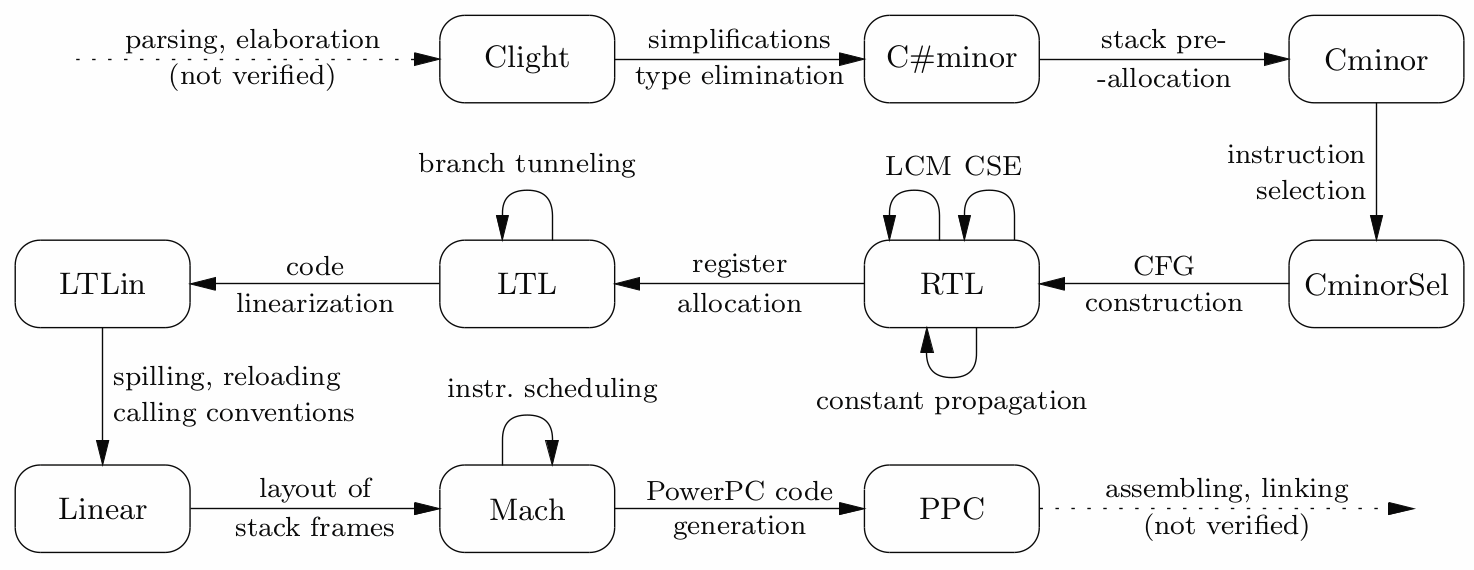
\includegraphics[scale=0.32]{images/compcert_pass.png}
\caption{Compilation routine of CompCert (Xavier Leroy~\cite{Leroy:2009:FVR:1538788.1538814}, Figure~1)}
\label{compcert_passes}
\end{figure}

CompCert has a standard compilation routine which is presented Figure~\ref{compcert_passes}. It has got some classic optimizations like constant propagation or elimination of common subexpressions. Performances of code produced by CompCert are correct, on PowerPC it reaches 90\% of the efficiency of \texttt{gcc} with optimizations at level 1.

CompCert verifies a theorem of correctness which certifies that every program compilable by CompCert will keep its semantic. More explicitly, every safe source program $S$ (\textit{safe} here means that all its code is well defined in ISO C 99) will be compiled in an assembly code $C$ which verifies the same properties than $S$.
In the case of a source program with undefined behaviour (in the semantic of CompCert C) we will have no guarantee on the correctness of the produced code.
For example an operation without semantic in CompCert is an access out of the bounds of an array.

\paragraph{Memory model of CompCert.}
\label{par:Memory model of CompCert}
CompCert uses an abstract representation of the memory for its semantics~\cite{compCert_memory_model}. This model is used to prove the correctness of the multiple compilation steps of CompCert. Therefore all the intermediary languages of CompCert share this memory model.

The memory is represented by blocks of finite size and each are given a block number $b$. These blocks are separated and to access a precise location in each block we use an offset $\delta$. Pointers are then represented by the couple $(b,~\delta)$. It is also possible to represent function pointers which are represented by pointers with negative block numbers $b$. It can be surprising that such abstract model of the memory can give us enough finesse to represent our SFI transformations. However the fact that memory blocks are disjointed is enough to isolate a part of the memory. Thus one these memory blocks will be reserved as the sandbox of our implementation.

\subsubsection{SFI with CompCert}
\label{ssub:SFI with CompCert}

We present an implementation of SFI with CompCert that was done by Joshua A. Kroll, Gordon Stewart et Andrew W. Appel~\cite{Kroll:2014:PSF:2708449.2708686}. The approach is composed of two parts, first of all SFI transformations are done in the intermediary language Cminor. We will then get a sandboxed Cminor code with the properties of SFI. The correctness theorem of CompCert guarantees that if the sandboxed Cminor is \textit{safe} in the definition of CompCert then the produced code will also verify the properties of SFI.
This way, the verifier present in the traditional approach is not necessary anymore since CompCert gives us equal guarantees. Hence this approach of SFI will not need a verifier in its TCB which is an advantage.

\paragraph{Cminor.}
\label{par:Cminor}

Cminor is an intermediary language created for CompCert. It is similar to a simplified version of C where we remove the type of the variables. Cminor was chosen for the SFI transformation because it is the lowest level language in the compilation steps of CompCert which is still architecture independent. This way, SFI transformations done in Cminor will be architecture independent as well. Moreover Cminor is also low level enough to be an intermediary language for other source language other than C. For these different reasons Cminor is the ideal candidate for the sandboxing operations of SFI.

\paragraph{Specification of the SFI transformation.}
\label{par:Specification of the SFI tranformation}
SFI techniques give us the following property. Any implementation of SFI should be able to transform any dangerous module into a module which respects the properties imposed by SFI. Therefore even for a semantically ill-defined module, CompCert-SFI is supposed to produce SFI compliant code.
In this case the sandboxed Cminor needs to verify these two properties:
\begin{itemize}
	\item the sandboxed Cminor confined all the memory accesses to its sandbox
	\item the sandboxed Cminor needs to be safe semantically in order to be able to use CompCert correctness theorem
\end{itemize}

This means that even if the source program is semantically ill-defined for CompCert, the SFI transformations need to make it semantically safe even if it modifies its behaviour.
However if the source program is already secure the SFI implementation will not modify its behaviour.

\paragraph{Masking in CompCert.}
\label{par:Masking in CompCert}
The CompCert-SFI uses the memory model of CompCert to prove that the SFI properties injected in Cminor still hold after the compilation. To represent the masking operation in the semantic of CompCert a native CompCert \textit{mask} function was created. This \textit{mask} function was axiomatized to be able to prove that the SFI transformations does not change the semantic of secure programs.
For example one of the axiom of the \textit{mask} function is ``If a pointer already points to the memory block of the sandbox then \textit{mask} does not change its value''.

\begin{figure}
\centering
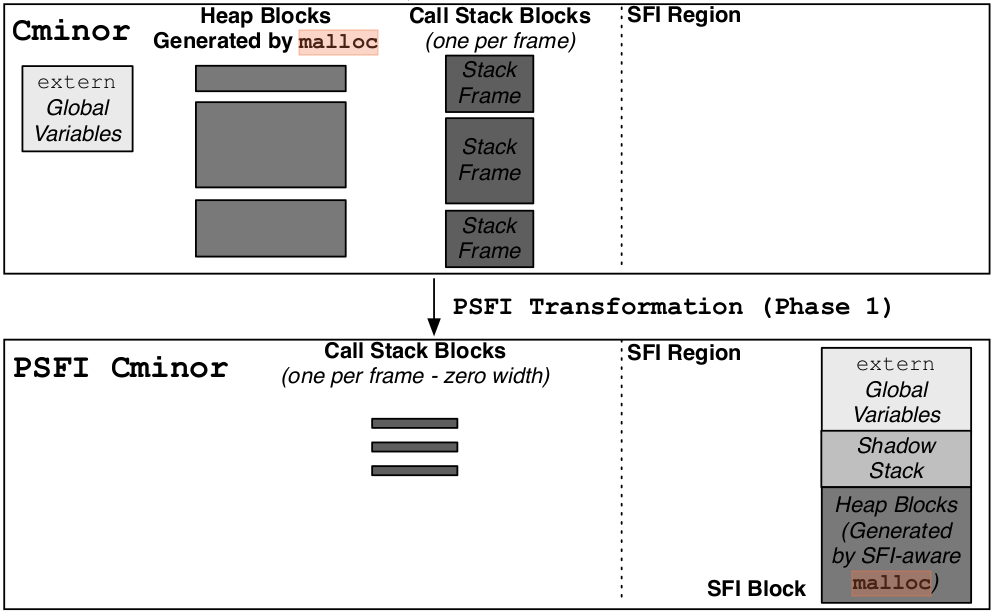
\includegraphics[scale=0.36]{images/psfi.png}
\caption{\textit{Sandboxing} of a module in CompCert (Joshua A. Kroll et al., Figure~1)}
\label{psfi}
\end{figure}

\paragraph{SFI transformations}
\label{par:SFI transformations}
There are two ways in CompCert Cminor to allocate memory. The first one is to use an external function like \texttt{malloc} otherwise you allocate frames in the stack. Then we need to ensure that the dangerous module Cminor can only allocate memory in the sandbox like in Figure~\ref{psfi}. Therefore CompCert-SFI will transform the dangerous Cminor with multiple steps:
\begin{itemize}
	\item \textit{Creation of a secondary stack}, this second stack will be created in the SFI area. Hence all the local variables of the dangerous modules will be stored in this second stack and will stay in their sandbox. To create such stack in the sandbox, we create a modified \texttt{malloc} function that will only allocate memory in the sandbox. This SFI-\texttt{malloc} will then be used to allocate the different frames of the secondary stack like in Figure~\ref{shadow_stack}. 
	\item \textit{Replacement of} \texttt{malloc}, like we said earlier an SFI-\texttt{malloc} was created that only allocates memory in the sandboxes. This SFI transformation will then replace all the classic \texttt{malloc} used with this SFI-\texttt{malloc} to confine the modules to their sandbox.
	\item \textit{Masking the memory accesses}, we inject the \textit{mask} function described earlier before all possibly dangerous instructions.
	\item \textit{Masking the function call}, memory areas are specially reserved to identify and control function pointers that could compromise the control flow of the program. Each memory area is dedicated to one authorized function of the protected program. Therefore the function pointers are redirected to these memory areas which we will control the interactions between the modules and the protected program.
	\item \textit{Production of semantically safe code}, we want that all the code produced by SFI to be semantically well defined in CompCert. For this, we modify the Cminor to remove all semantically ill-defined code. For example, all the local variables which appear in the modules are initialised, we add runtime checks to prevent any division by zero or we verify that function calls match an existing function signature.
\end{itemize}

\begin{figure}[!ht]
\centering
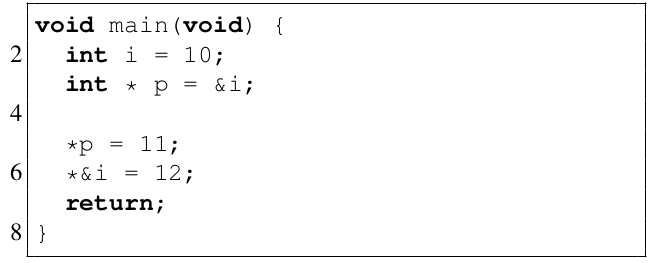
\includegraphics[scale=0.33]{images/before_shadow.png}
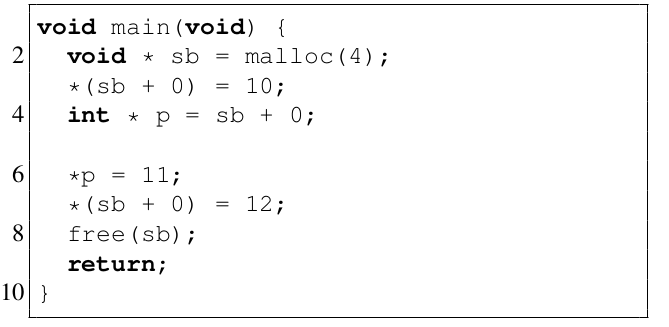
\includegraphics[scale=0.33]{images/after_shadow.png}
\caption{Using \texttt{malloc} to allocate memory for the frames (Joshua A. Kroll et al.)}
\label{shadow_stack}
\end{figure}

\subsubsection{Evaluation of the approach}
\label{ssub:Evalutation of the approach}
First of all a strong point of this approach is that it has a small \textit{Trusted Computing Base}. For the CompCert-SFI to be valid it is only necessary to trust that our SFI transformations which were not proven (like the axiomatized \textit{mask} function) does not change the behaviour of the dangerous modules. Moreover we need to trust CompCert, especially the small pieces which are not proven like the proof assistant Coq or the assembler. \\
Another asset is that the absence of verifier of the approach which remove the necessity to develop a different verifier for every architecture targeted. Furthermore the SFI transformations are portable on every architecture supported by CompCert. Cminor is also a high level language, therefore the SFI transformations can still benefits from the optimization operations of CompCert and speed up the module. \\
The performances obtained during the experiments are similar to a compromise between \texttt{gcc -O0} and \texttt{gcc -O1} for ARM a and x86-32. If we compare the efficiency with CompCert without SFI we have a drop of 21.7\% on x86-32 and 16.8\% on ARM.

However CompCert-SFI also got some downsides. First, the correctness property of CompCert does not apply for concurrent programs. Indeed CompCert does not have an operational semantic for multi-tasking programs which means we cannot ensure the SFI properties in this case. Also the CompCert-SFI approach forces us to compile the dangerous module to have sandboxed executables.
Whereas in the traditional SFI the dangerous modules can be distributed as binaries, then we only need to have the approval of the verifier to execute them without dangers. \\


\subsection{Limit of SFI}
\label{sub:Limits of SFI}

We saw that SFI techniques confine jumps in the code differently depending of the addressing mode. For a direct addressing, the generator just rewrites directly the targeted address by replacing the most significant bits with the tag of the sandbox. For indirect addressing we added some runtime sandboxing operations to make sure that the targeted address stored in the register would be in the sandbox. There is also another way to make a jump which uses an address stored in the stack: the \texttt{ret} instruction. Since \texttt{ret} does not use any register we can't use our sandboxing operation here. We could just mask the value stored in the stack but like we mentioned Chapter~\ref{par:NaCl_32} this solution is vulnerable to race conditions. Indeed we can't guarantee that the value stored in the stack will not be overwritten by another thread between the runtime check and the execution of \texttt{ret}. Therefore the code is vulnerable to Returned Oriented Programing (ROP) attacks which will be presented in details Chapter~\ref{sub:rop_attack}. These attacks overwrite the return addresses located in the stack in order to modify the control flow of the program and possibly execute malicious code. 

In the works presented only NativeClient~\cite{Yee:2010:NCS:1629175.1629203} addresses this issue. The idea is to remove all \texttt{ret} instructions and replace them by the composition of a \texttt{pop} and a \texttt{nacljmp} which is the SFI \texttt{jmp}. 
This simple solution works but the modern processors use numerous optimizations linked to the use of \texttt{ret} instructions. Replacing \texttt{ret} instructions greatly decreases the efficiency of the programs. 
Thus we propose in the following section a more flexible and efficient solution to protect return addresses against the famous ROP attacks and this solution could complete the SFI implementations presented perfectly. 

\newpage
\section{Overview of the approach}
\label{sec:Overview of the approach}
	Many attacks on software aim at diverting the control flow of the targeted program. Among those, \textit{Returned Oriented Programming} (ROP) attacks specifically try to overwrite the return addresses.
By doing so the attacked function will return to a malicious piece of code that will get executed.
Stack overflow is an example of such ROP attacks.
We propose a solution against ROP attacks which combined with SFI would protect from most of control-flow interference attacks.
Inspired from SFI techniques we aim to prevent any overwriting of the return addresses. To do so we need to know these return addresses locations in the memory. Therefore our approach consists of modifying the stack structure in order to have a way to distinguish the return addresses locations. With this knowledge we will be able to put a mask, as in SFI, before every dangerous write instructions and prevent any ROP attack.


\subsection{ROP attacks}
\label{sub:rop_attack}

	We want to protect our program against ROP attacks. These attacks are directed against the stack and especially the function return addresses located in the stack.
We will begin by a short introduction about the mechanisms behind the stack. Then we will explain how ROP attacks work with the example of a classical buffer overflow.

\subsubsection{The stack}
\label{ssub:The stack}
	The stack is a specific area of the memory of a program. The memory allocated to a program is divided among multiple areas like the stack (which we are going to detail), the heap (where we put dynamically allocated or global variables) and the code is also allocated in a specific area.
The stack is composed of frames and each of them are related to a function being executed. Frames are piled up on the stack following the FIFO rule (\textit{First In First Out}). Explicitly, every time a function is called, a new frame is created and placed on the top of the stack. Reciprocally when a function terminates its frame will be popped out of the stack.
Frames contain multiple kind of data related to their function like local variables, parameters of the function and return addresses. Return addresses indicates the point of execution to return to after a function terminates. When popping a frame the program is supposed to execute the code at the address matching the value contained in the return address.
ROP attacks aims to overwrite these return addresses which enables them to execute malicious code hidden in another part of the memory instead of continuing the normal flow of the program.

\subsubsection{Buffer overflow}
\label{ssub:Buffer overflow}

Stack overflows are the most popular ROP attacks \textcolor{green}{ref} . In Figure~\ref{buffer_overflow_code} we can see an example of buffer overflow written in C.
The goal of this code is to execute the function called \textit{evil\_code()} which just prints ``Argh, we got hacked!\textbackslash{n}'' line~6 of Figure~\ref{buffer_overflow_code}. The function \textit{evil\_code()} should not be executed in our program, we suppose it is never called.
The code was compiled with \textit{gcc -m32 -fno-stack-protector} to remove all stack protections used by gcc. The output of the code of the successful buffer overflow can be seen in Figure~\ref{output_buffer}.
\begin{figure}[!ht]
\begin{lstlisting}
void evil_code() {
	printf("Argh, we got hacked!\n");
}

void foo(char* input){
	char buf[1];
	... code ...
	strcpy(buf, input);
	... code ...
}
\end{lstlisting}
\centering
\caption{Example of buffer overflow in C}
\label{buffer_overflow_code}
\end{figure}

We printed out the stack before and after the attack to have a better comprehension of the attack.
We see in the Figure~\ref{output_buffer} the consequences of the buffer overflow in red. The stack was overwritten and the return address was modified to the address of \textit{evil\_code()} which code was successfully executed.

The vulnerability resides in the function \textit{strcpy} line~8. \textit{strcpy} just copies characters one by one until it finds ``0''(which corresponds to the end of a string) in the source string. However our source string can contain many more characters than \textit{buf} is supposed to have. 
Indeed \textit{buf} is declared line~6 as an array of 1 character and our source string is the argument that we give to the program.
If the source string is bigger than the destination \textit{strcpy} will just continue to write the source string over others variables location in the stack and possibly reach the return address.
The variable \textit{input} has the value of the parameter we give to our program and is the string we are supposed to copy in \textit{buf}.
After few tries and fails we found the correct parameter to successfully do the buffer overflow. This input can be seen on the first line of Figure~\ref{output_buffer} which is \textit{python -c 'print 13*"a"+"\textbackslash{x7b}\textbackslash{x84}\textbackslash{x04}\textbackslash{x08}}` or \textit{aaaaaaaaaaaaa\textbackslash{x7b}\textbackslash{x84}\textbackslash{x04}\textbackslash{x08}}\\
In our example we filled the stack with ``a'' which corresponds to ``61'' in ASCII until we reached the return address.
We can see the consequence of the attack in the output Figure~\ref{output_buffer}, where the stack is full of ``61'' after executing \textit{strcpy}.
When we reached the return address we overwrote it with the address of \textit{evil\_code} which was \texttt{0x0804847b} given on the second line of Figure~\ref{output_buffer}.
This way, the next instruction that will be executed after \textit{foo} finishes will be the function \textit{evil\_code}.
At the end of the program we can see that we get a \textit{Segmentation fault (core dumped)}, which is normal because we messed up the stack when we overwrote is with ``a''. But since we managed to execute \textit{evil\_code} the attack is still successful. \hfill \break

Even though the buffer overflow was a basic one, it still happens to see the usage of vulnerable functions like \textit{strcpy} in the industry.
Furthermore there are much more sophisticated ROP attacks which are much more effective as witnessed by security vulnerability reports.
Before, classic ROP attacks tried to execute some malicious code that was inserted manually in the stack or in the heap. But nowadays most system render their stack and their heap non executable which prevents the classic ROP attacks.
However modern ROP attacks are now able to create malicious code from different pieces found in the program or in the libraries used. The most famous one is called \textit{return-to-libc}~\cite{BRSS08}\cite{S07} attack which pieces of code from the \textit{libc} library to create malicious code. Then the attacker still try to deviate the control flow of the program through return addresses to the malicious code just assembled with \textit{libc} code.

\begin{figure}[!ht]
\textcolor{gray}{terminal\$~} ./buffer \$(python -c 'print 13*"a"+"\textbackslash{x7b}\textbackslash{x84}\textbackslash{x04}\textbackslash{x08}"') \\
\textcolor{red}{Address of evil\_code = 0x0804847b} \\
Stack before: \hfill \break
0xf7712000    \hfill \break
0xff957998    \hfill \break
0xf7593d26    \hfill \break
0xf7712d60    \hfill \break
0x0804868c    \hfill \break
0xff957978    \hfill \break
0xf7593d00    \hfill \break
0xf7713dc0    \hfill \break
0xf77828f8    \hfill \break
0xff957998    \hfill \break
0x08048510    ~~~~~~~~~~~~~~~~\textcolor{blue}{//Return address of \textit{foo}}\hfill \break
              \hfill \break
Stack after : \hfill \break
0xff958161    \hfill \break
0xff957998    \hfill \break
0xf7593d26    \hfill \break
0xf7712d60    \hfill \break
0x0804868c    \hfill \break
0xff957978   			   ~~~~~~~~~~~~~~~~\textcolor{blue}{//Buffer overflow}\hfill \break
\textcolor{red}{0x61}593d00~~~~~~~~~~~~~~~~\textcolor{blue}{//``a''   } \hfill \break
\textcolor{red}{0x61616161}~~~~~~~~~~~~~~~~\textcolor{blue}{//``aaaa''} \hfill \break
\textcolor{red}{0x61616161}~~~~~~~~~~~~~~~~\textcolor{blue}{//``aaaa''} \hfill \break
\textcolor{red}{0x61616161}~~~~~~~~~~~~~~~~\textcolor{blue}{//``aaaa''} \hfill \break
\textcolor{red}{0x0804847b}~~~~~~~~~~~~~~~~\textcolor{blue}{//"\textbackslash{x7b}\textbackslash{x84}\textbackslash{x04}\textbackslash{x08}",  \textit{evil\_code} address \\}
\\
Argh, we got hacked! ~~\textcolor{blue}{//Success! \textit{evil\_code} was executed}\\
Segmentation fault (core dumped)
\caption{Output from buffer overflow example}
\label{output_buffer}
\end{figure}


\subsection{Description of the approach}
\label{sub:Description of the approach}
	We want to protect programs against ROP attacks like the buffer overflow seen previously. We want to prevent any return address from being overwritten illegally. The only moment they should be written over is during a function call routine.
We want to be able to add runtime checks in the code like SFI, therefore we need to be able to check if an address is the location of a return address. 

The biggest difficulty is to be able to know if a location in the stack corresponds to a return address or not. Indeed the stack grows through function calls which pile up stack frames. 
These frames are constructed dynamically depending of the function, hence the locations of return addresses are not easily known.
As it is we do not have enough information to correctly protect return addresses since we do not know precisely where they are located.

Several solutions exists against this issue. We could for example add a lot of meta-data during the compilation to have extra information and then effectively protect the return addresses. Another solution is to create a second stack called \textit{shadow stack}. We would then have complete control over the \textit{shadow stack} which allows us defend against ROP attacks.
\textcolor{green}{maybe expose the cons of these approaches from our point of view}

Our solution is to modify the current stack structure to be able to know the return addresses locations easily. The main idea is to fix a constant offset $n$ between return addresses allowing us to exactly know where a return address is located relative to the others. We will explain thoroughly the approach that we want to apply in the following section.

\subsubsection{Proposed solution}

\paragraph{Fixing return addresses locations and stack alignment.}
\label{par:Fixing return addresses locations}

We want to be able to decide if a pointer points to a return address at runtime. With this knowledge we will be able to detect if an instruction may compromise our program.
The idea is to modify the stack layout in order to have a constant offset $n$ between neighbouring return addresses. This way we know that the neighboring return addresses are always located at a distance $n$ from a frame return address. Furthermore all the other return addresses are separated by a distance which is necessarily a multiple of $n$.
For example suppose that we know the location of a return address, we call this location $c$.
Since all neighboring return addresses are separated by the exact amount $n$, we know that the following return addresses locations will be $c+k*n$ with $k>0$. Reciprocally the previous return addresses will be located at $c-k*n$ with $k>0$.\\
Thus we can generalize the two previous relations and for every return address location \textit{a} we will have the relation $a~mod~n = c$.

The next hurdle is to choose $n$ and $c$ cleverly. 
For $n$, the most important thing is that frames have enough space to store all the needed data. Therefore we define the value of $n$ as the biggest frame size of all the functions in a program.
If the return addresses are separated by this amount we are sure that every function will have enough space in the stack for its frame. \\
Afterwards we have to define $c$. The best way that we found is to modify the stack in order to have the first return addresses location to be equal to $c$. If we are able to do such a thing, we can also easily define the value of $c$ and for simplicity we would like to have $c~mod~n = 0$

The Figure~\ref{idea_stack} pictures the transformation we want to apply to the stack. On the left we have represented an usual stack with return addresses all over the place.
Since these locations are almost random it's really difficult to pinpoint their location. After transforming the stack (stack on the right) we can see that the different addresses are separated by the same constant $n$.

We have two relations about return addresses location:
$$[\forall a\in Ret\_locations,~a~mod~n=c]\text{ and }[c~mod~n=0]$$
$Ret\_locations$ is the set containing all the locations of return addresses.
We can combine our two properties and we obtain:
{\Large $$\forall a\in Ret\_locations,~a~mod~n=0$$}

\begin{figure}[!ht]
\centering
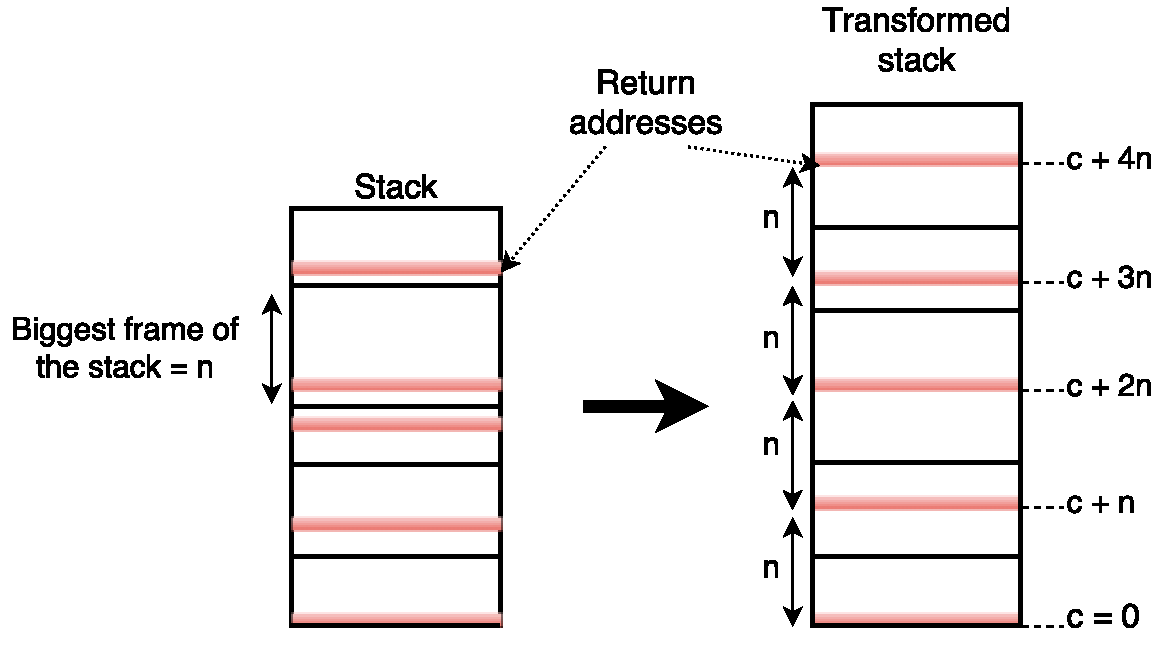
\includegraphics[scale=0.6]{images/idea_stack.pdf}
\caption{Stack modifications}
\label{idea_stack}
\end{figure}

\paragraph{Detection of dangerous instructions.}
\label{par:Detection of dangerous instructions}

The second step is to detect every possibly harmful instructions to return addresses. We consider as dangerous every instruction that can freely write to the memory. Our approach is mainly related to the C language.
In C, instructions that fit such criteria are assignment to pointer dereference in the form of  \textit{(pointer)*~=~value} or \textit{(pointer+offset)*~=~value}. \\
In the previous example of buffer overflow Figure~\ref{buffer_overflow_code}, the vulnerability resides in the function \textit{strcpy} line~12. To pinpoint the dangerous instruction let's check the source code of \textit{strcpy} Figure~\ref{strcpy} from Apple.
We can see in the \textit{while} loop line~10 that \textit{strcpy} copies characters one by one from the source string \textit{s2} to the destination \textit{s} until it finds a character equals to \textit{0}.
To copy the characters, \textit{s} and \textit{s2} are pointers which initially point to the memory area of the destination and the source string. Then until it finds a character matching \textit{0} the value pointed by \textit{s2} is copied to the location pointed by \textit{s} and the pointers are incremented. The harm happens when the source \textit{s2} is much longer than the destination. In this case we continue to copy to the location pointed by \textit{s} even if the memory written to does not belong to the destination string anymore.\\
In this example we see clearly that it's the pointer dereferencing that allows one to write directly in the memory. For that reason we target such type of instructions in our approach.

\begin{figure}[!ht]
\begin{lstlisting}
char * strcpy(char *s1, const char *s2) {
	char *s = s1;
	while ((*s++ = *s2++) != 0)
		;
	return s1;
}
\end{lstlisting}
\centering
\caption{\textit{strcpy} source code from Apple}
\label{strcpy}
\end{figure}

\paragraph{Securing dangerous statements.}
\label{par:Protection around dangerous statements}

Finally when we have detected all the dangerous statements we transform the module code. Before each of this dangerous statement we add a protection mechanism similar to masking in SFI. The algorithm of the check is represented in Figure \ref{runtime_check}: \\
	\begin{enumerate}
		\item We check if the address is in the stack. Return addresses only exist in the stack, we do not need to concern ourselves with the other accessible memory area: the heap.
		\item If the address is in the stack we check if the target address $a$ verifies our equality $a~mod~n=0$. If it does then it's a return address location.
		\item If a target address abides by the two previous condition, it's an illegal instruction and we make the program crash. If it does not then the program just continue to run like normal.
	\end{enumerate}
We want our implementation to respect the property of transparency, if a program is safe then our transformation does not modify its behaviour.

\begin{figure}[!ht]
\centering
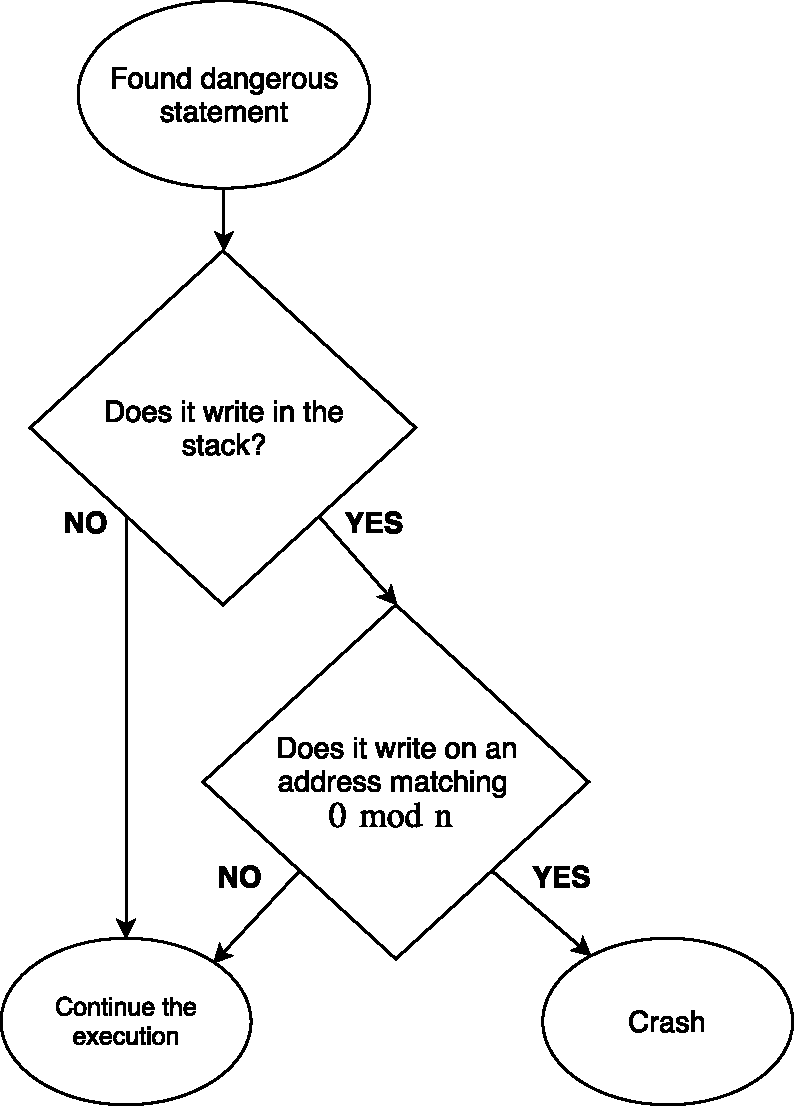
\includegraphics[scale=0.6]{images/runtime_check.pdf}
\caption{Runtime check algorithm}
\label{runtime_check}
\end{figure}

\hfill \break 
	To sum it up, our approach aims to have an easy way to know return addresses location and then add a check at runtime before every dangerous instruction to prevent illegal writing on return addresses location.
To do this we divided the approach into four phases:
\begin{enumerate}
	\item Fix stack frames size
	\item Align the stack
	\item Detect dangerous statements
	\item Secure the dangerous statements
\end{enumerate}


\subsection{Security properties}
\label{sub:Security properties}
	The approach we propose is composed of four phases, to get the confidence that our idea is effective in protecting return addresses we are going to formalize the properties we expect from each phase. 
Furthermore like we pointed earlier, we are going to work with the certified compiler CompCert.
The ideal way to be sure of our idea would be to prove it with Coq the proof assistant the language used to build CompCert.
By working with these tools we hope that eventually we will be able to prove some security guarantees brought by our approach.

\begin{enumerate}
	\item \textbf{Fixed stack frames size}
		\begin{itemize}
			\item Return addresses locations are all separated by a constant offset $n$ bigger or equal to any frame of the stack
		\end{itemize}
	\item \textbf{Stack alignment}
		\begin{itemize}
			\item The first return address location $c$ of the program verifies $c~mod~n=0$
		\end{itemize}
	\item \textbf{Detection of memory write statements}
		\begin{itemize}
			\item Every statement of the analysed code that might modify the stack memory state is detected
		\end{itemize}
	\item \textbf{Securing memory write statements}
		\begin{itemize}
			\item The protection will trigger an error behaviour if we try to write on a protected address
		\end{itemize}
\end{enumerate}

Combined, properties 1. and 2. give us the guarantee that the least significant bits of all the return addresses location will verify $a~mod~n=0$ with $n$ the fixed offset between return addresses.
Basically we make it so the protection mechanism prevents any write on addresses located in the \textbf{stack memory area} and verifying $a~mod~n=0$.

\hfill \break 
Another property we did not mention yet is that all our transformations need to be transparent. In other words, if we apply our methods on a program which is already safe then its behaviour is not affected. We will explain how we ensure this property more thoroughly in Chapter~\ref{sec:implementation}.

\hfill \break 
For these properties to always hold true we need to place some conditions which we are going to list in the following section. Our approach guarantees that if all the properties mentioned are fulfilled the program will be protected against any ROP attack.

\subsection{Analysis of the approach}
\label{sub:Analysis of the approach}

\subsubsection{Conditions}
\label{ssub:Conditions}

The solution we have just presented can bring very strong security properties against ROP attacks. However for this approach to work we need certain hypothesis to be true. Indeed some of the properties enumerated before are invalidated after certain operations.

\paragraph{Stack modifications.}
\label{par:Stack modifications}
Every operation that disrupts the stack structure may nullify our property that says ``every return addresses are separated by a fixed offset''. For example x86 architecture use the ESP register to keep track of the stack growth. If we fiddle with it we may introduce a shift in the return addresses location. Then our runtime check of the return addresses locations property $a~mod~n=0$ would not be relevant anymore.
		For example, the Figure~\ref{inline_assembly} shows a piece of inline assembly which disrupts the stack line~2. Inline assembly allows one to put some assembly code in the middle of C code. Here the assembly decrements the stack pointer stored in ESP. By doing so the stack will be shifted by an amount of 50 bytes and our formula to the locations of return addresses will not be correct anymore.

\paragraph{Insecure libraries.}
\label{par:Insecure libraries}

For our approach to work we need to have all dangerous write statements to contain our runtime checks. Hence all executed code must have been compiled with our transformation. For example, the \textit{glibc} library of C contains multiple insecure functions like \textit{printf, strcpy\dots} Furthermore those flawed functions are common vulnerabilities for \textit{buffer overflows} attacks which are a type of ROP attack. To avoid this issue we would need to rewrite the glibc or compile it with our tools.

\paragraph{Modules need the same offset.}
\label{par:Modules need the same offset}
If a program uses multiple modules or library they need to be compiled with the same offset $n$. Indeed if the offset of the different modules are different we cannot use the previously defined relation $a~mod~n=0$ cannot be used anymore. Thus it is not possible to easily know if a location corresponds to a return address.

\begin{figure}[!ht]
%asm(''sub $50, %esp'');
\textcolor{green}{TODO substitute with the right syntax when finished}
\begin{lstlisting}
int foo(int a) {
	asm(``\$sub 50, \%esp'');
	//This line does the operation ESP = ESP - 50
	//This disrupts the stack layout we establish in our transformation
	printf("Hello world!");
}
\end{lstlisting}
\centering
\caption{C inline assembly}
\label{inline_assembly}
\end{figure}

\subsubsection{Discussion}
\label{ssub:Discussion}
	We have presented the principle of our approach in this chapter. Then we mentioned some necessary conditions for our solution to work properly. In this section we are going to discuss about the pros, cons or remarks about the proposed solution.

	The benefits of our transformation is clear, any code compiled with a compiler enforcing our methods is unable to interfere with the control flow of our program through return addresses.
	Furthermore if we combine our solution with the SFI presented earlier we can have some strong security properties on the execution of dangerous modules with our main program.
Our approach may also have some impact on portability and efficiency:

\paragraph{Architecture dependant.}
\label{par:Architecture dependant}
Our solution depends a lot of the stack layout of the program.
Indeed fixing the size of the frames requires us to modify the original stack layout.
Therefore since the stack layout vary depending of the architecture and compiler you are using, the modifications that have to be done are also different.
We can then easily comprehend that we would need a different implementations for every existing stack layout.
Moreover since these layouts can be really different it might be quite complicated to implement our solution on certain of them.
In the implementation we present after we focus solely on x86-32 architecture with the compiler CompCert.

\paragraph{Memory consumption.}
\label{par:Memory consumption}
Since we are fixing the size of the frames instead of having dynamic sizes the memory usage of the stack is bigger. We have the issue of choosing an adequate size for the frames in our solution. The easiest one is to take the maximum frame size of the program as the constant size for all the frames. The downside is that we might have a memory usage explosion from our stack.
We did not encounter any issue about memory during the tests we did but the impacts may be visible on especially big programs. It might be interesting to study the efficiency of our approach on the growth of the stack.

Despite the cons presented we believe the benefits we gain from this method is worth it.
We are going to present in the following section the implementation we made based on the ideas we introduced here. This implementation was made with the compiler CompCert for the x86-32 architecture. We are targeting programs written in C, which explains that all the examples we used were related to the C language.


\newpage
\section{Implementation}
\label{sec:implementation}

For the implementation we work with the compiler CompCert. CompCert already has an implementation of SFI presented earlier. Thus if we could combine our approach with the SFI, any program compiled with CompCert would have strong security guarantees. Furthermore CompCert is written with the Coq proof assistant, our implementation then paves the way for a formal proof of security properties. In this section we explain in details how to enforce our approach and the different choices we made during the process.

	Our approach is separated in four phases: ``Fixed stack frames size'', ``Stack alignment'', ``Detection of memory write statements'' and ``Evaluation of the implementation''. We are going to detail the implementation of these phases in the following sections. These transformations are deeply linked to the stack layout, hence to have a better understanding we are going to start by introducing the CompCert stack structure.

\subsection{CompCert stack}
	The layout of the stack is dependent of the architecture and the compiler/interpreter used. For the sake of comprehension of the future sections we describe here the stack layout of x86-32 in CompCert.
The stack layout of CompCert x86-32 is pictured in Figure~\ref{stack_layout}.
First of all we can notice that the stack grows downwards, it means that the stack grows from the highest addresses to the low ones.
As we can see the usual data are stored in this stack like local variables, parameters, register states and the return address.

\begin{figure}[!ht]
\centering
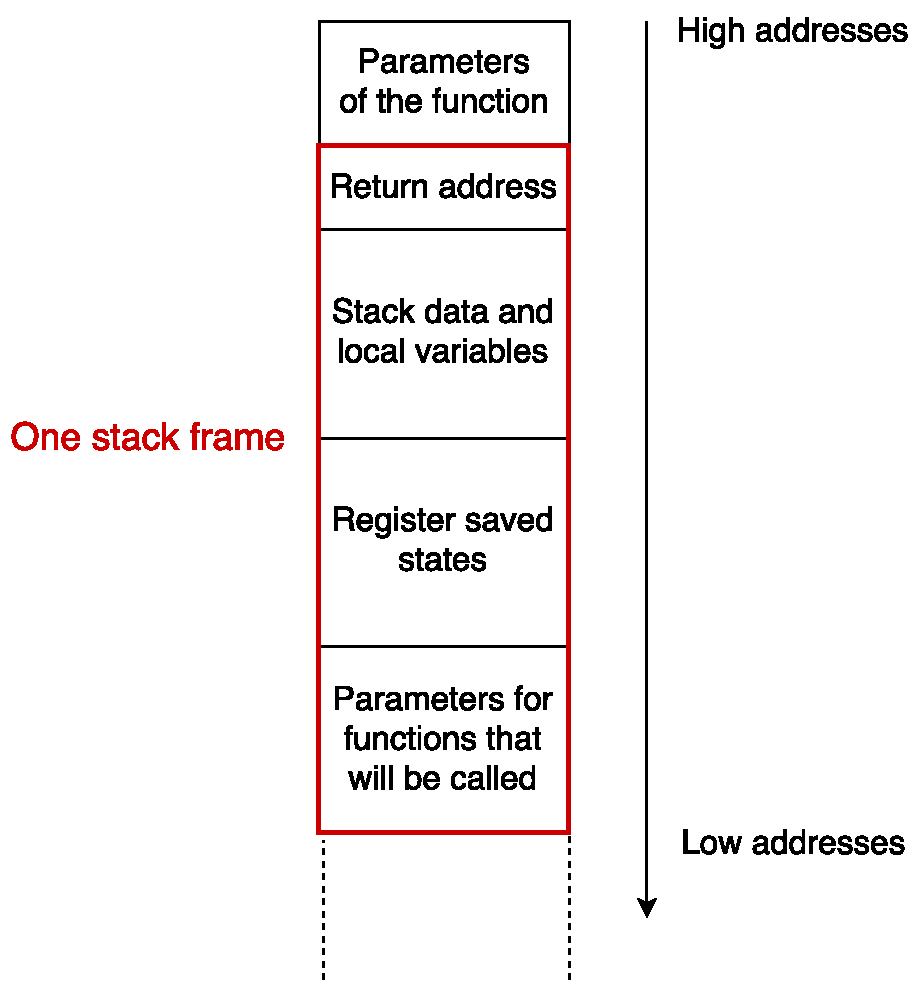
\includegraphics[scale=0.55]{images/stack_layout.pdf}
\caption{CompCert x86-32 stack layout}
\label{stack_layout}
\end{figure}

Each frame is built when a function is called, the different steps related to the creation of a frame is called \textit{function call routine}.
CompCert function call routine is described in the Figure~\ref{call_routine}. Each phase of the function call routine of the Figure~\ref{call_routine} is explained just here:
\begin{enumerate}
	\item Write the return address
	\item Allocate enough memory for the rest of the stack frame
	\item Save registers states in the stack
	\item Execute the function body (use the memory for local and stack data)
	\item When calling another function, place its parameters at the end of the stack and repeat the process
\end{enumerate}

\begin{figure}[!ht]
\centering
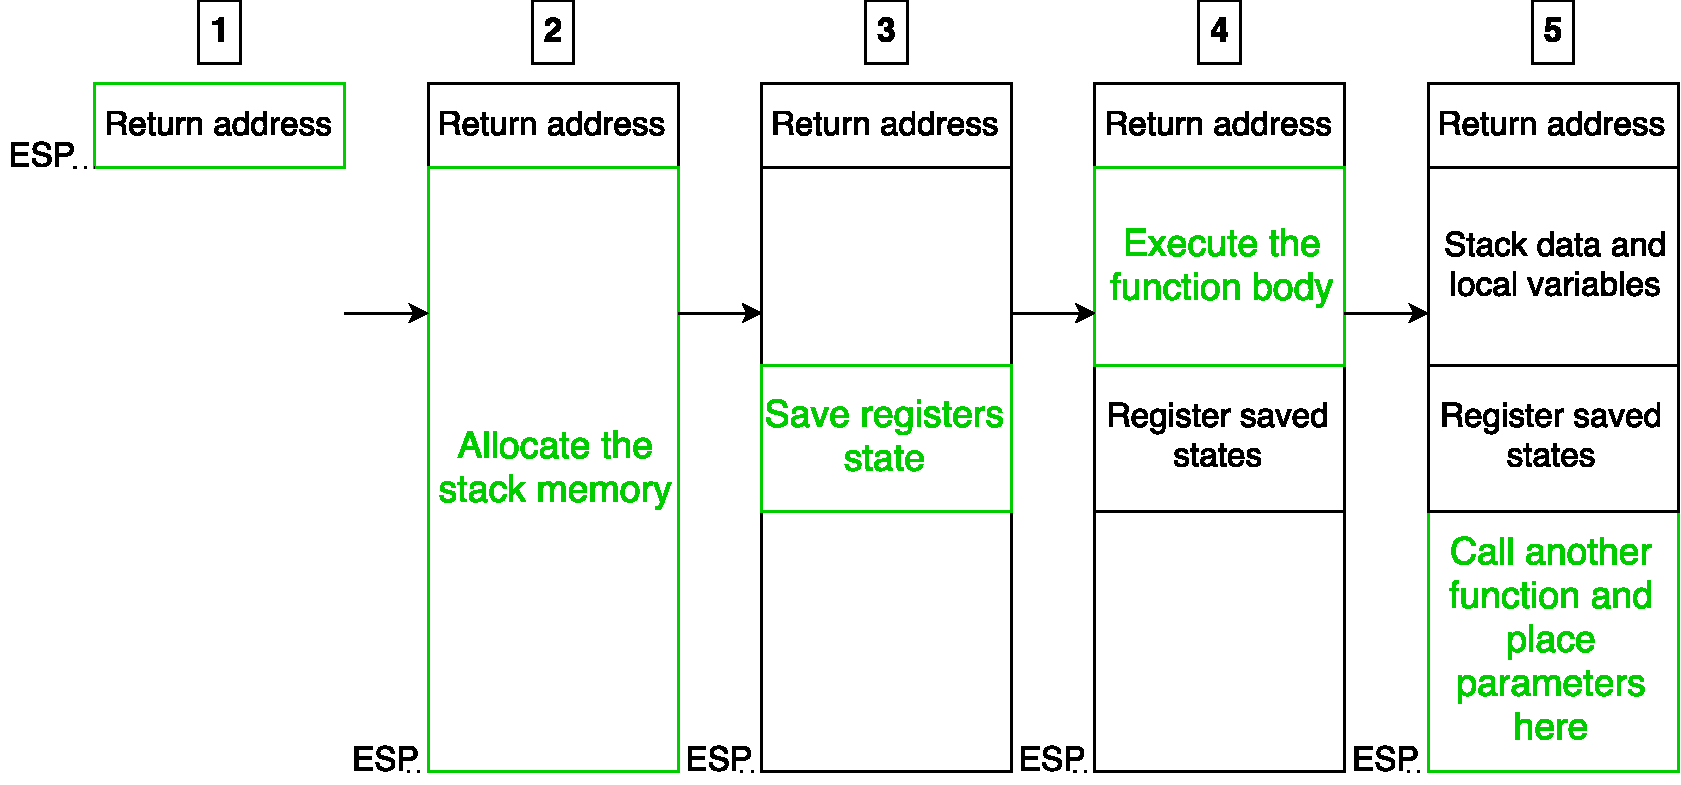
\includegraphics[scale=0.55]{images/call_routine.pdf}
\caption{CompCert function call routine}
\label{call_routine}
\end{figure}

When returning from a function, the return routine is pretty much the opposite:
\begin{enumerate}
	\item Restore registers state
	\item Deallocate the stack until the return addresses
	\item Pop the return address memory and jump to the value stored in it
\end{enumerate}


\subsection{Fixed stack frames size}
During this phase we want to ensure these two properties:
\begin{itemize}
	\item Return addresses locations are all separated by a constant offset $n$ bigger or equal to any frames of the stack
\end{itemize}

\paragraph{Fix the frames size.}
\label{par:Fix the frames size}

Fortunately in the function call routine of CompCert the return addresses are always at the top of their frames.
This particularity makes the task easier, indeed, since the location of the return address is fixed in the stack we can simply fix the size of the frames to have a constant offset between the return addresses. \\
To modify the stack layout of CompCert we just need to modify the record describing the frames presented Figure~\ref{frame_record}. In our case the record has different fields like the size of the whole frame and the offset of the different data of the stack. Hence we give to the field it \textit{fe\_size} line ~2 a constant $fe\_size=n$ which will be a power of two bigger than its previous value. We also need to keep the return address at the bottom of the frame (the stack grows downwards). Thus we have $fe\_ofs\_retaddr=n-4$ line~4 because the return address is four bytes long. The locals and stack data will then naturally fill the extra space left by the shifted return address like shown Figure~\ref{frame_transform}.

\begin{figure}[!ht]
\centering
\begin{lstlisting}[language=Caml]
Record frame_env : Type := mk_frame_env {
  fe_size: Z;
  fe_ofs_link: Z;
  fe_ofs_retaddr: Z;
  fe_ofs_local: Z;
  fe_ofs_int_callee_save: Z;
  fe_num_int_callee_save: Z;
  fe_ofs_float_callee_save: Z;
  fe_num_float_callee_save: Z;
  fe_stack_data: Z
}.
\end{lstlisting}
\caption{CompCert x86-32 frame record}
\label{frame_record}
\end{figure}

In Figure~\ref{frame_transform}, we present the transformation of the CompCert frame to a new frame with a fixed size equal to $n$. We can see that the stack data and locals part have increased and filled the empty space further in the bottom.

\begin{figure}[!ht]
\centering
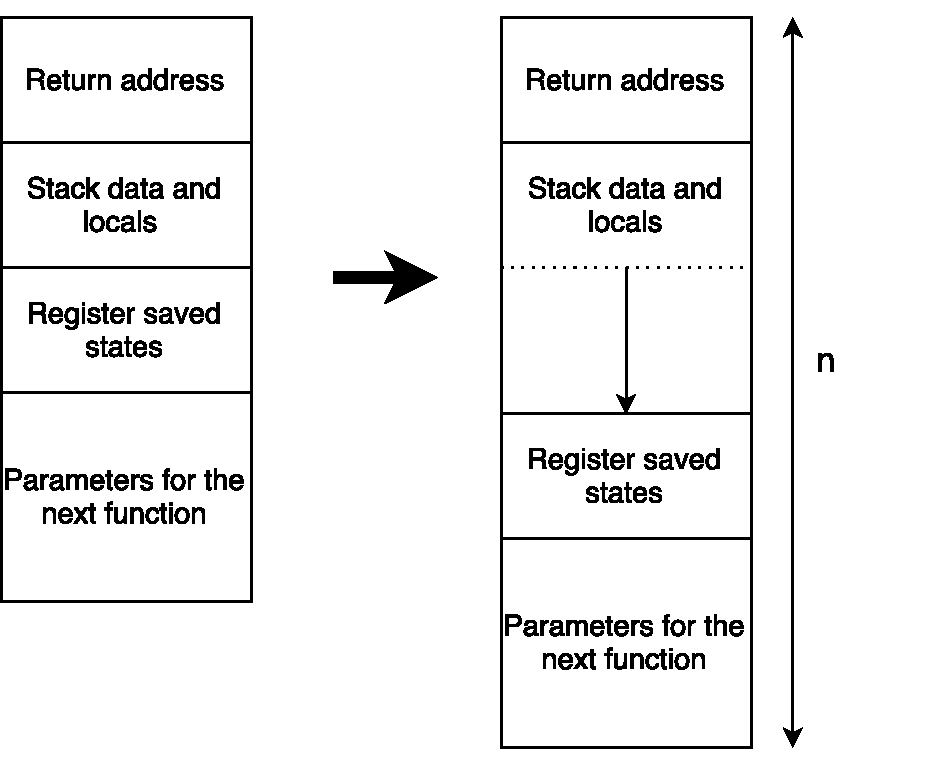
\includegraphics[scale=0.6]{images/frame_transform.pdf}
\caption{Transformation of CompCert frame}
\label{frame_transform}
\end{figure}

\paragraph{Choice of frames size.}
\label{par:Choice of frames size}

We chose to limit the choice of the frames size to powers of two. Indeed, since addresses are written in binary having a power of two as constant offset will ease the runtime checks implementation. By using powers of two, all the return addresses will have the same least significant bits. For example if the first return address location is \texttt{0xffffff910} (in hexadecimal) and our constant frame size is $2^8 = \texttt{0100}$ (in hexadecimal). Then all the following return addresses locations will be \texttt{0xfffff810} (the stack grow downwards), \texttt{0xfffff710}, \texttt{0xfffff610}\dots And their least significant bits are actually always equal to \texttt{10}. This particularity will help during the phase of runtime checks that we will explain in Section~\ref{sub:implem_check_address}.

To prevent having compiled programs with too small stack frame, we added in CompCert a check. This test verifies that the chosen size is bigger than any dynamically calculated one. If not, the compilation fails. This way the chosen size corresponds to the smallest power of two which is bigger or equal to any dynamically calculated frames size of the program.

We can see in Figure~\ref{stack_transform} the effect of our implementation. 
The left stack is the usual layout of CompCert stacks with the return addresses located at the top of the frames. We call $F_{size}$ the size of the biggest frame of the whole program.

For our transformed stack we have to chose a fixed size for the frames and it needs to be a power of two, bigger or equal to $F_{size}$. In Figure~\ref{stack_transform} we chose $2^8$ to continue the examples we gave before.
We can see that the stack on the right has fixed size frames equal to $2^8$ and the return addresses are all separated by the same offset dues to CompCert stack layout.
The implementation effectively fulfills the property of having constant offset between return addresses.
Furthermore we can see that the location of the return addresses are \texttt{0xfffff910}, \texttt{0xfffff810}, \texttt{0xfffff710}\dots
Hence all the return addresses have the particularity of always having the same least significant bits (\texttt{10}). This particularity will be used later for the implementation of the protection mechanism.

\begin{figure}[!ht]
\centering
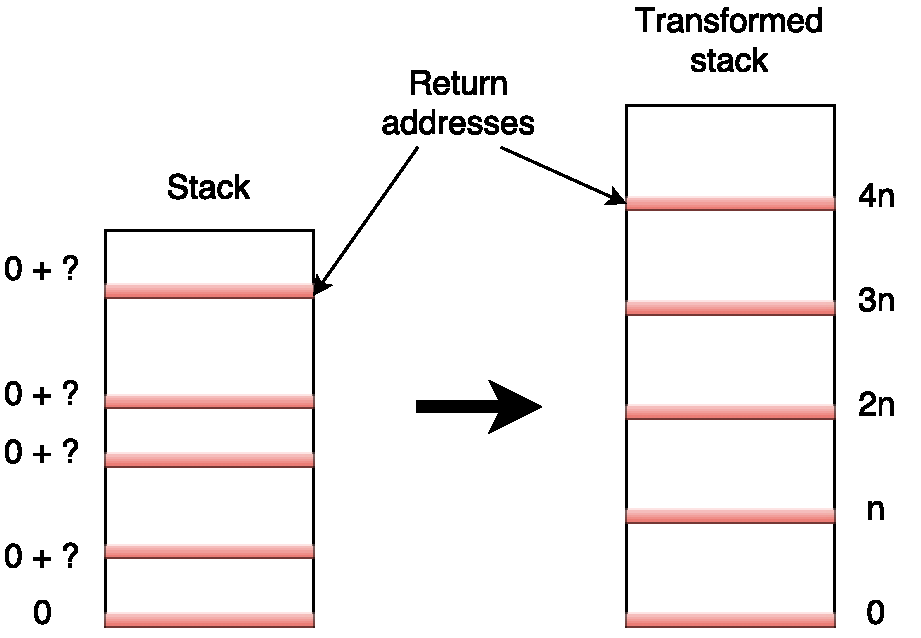
\includegraphics[scale=0.6]{images/stack_transform.pdf}
\caption{Fixing the size of CompCert stack frames}
\label{stack_transform}
\end{figure}

\subsection{Stack alignment}

The implementation in this section has to do a transformation that makes the following property true:
\begin{itemize}
	\item The first return address location $c$ of the program verifies $c~mod~n=0$
\end{itemize}

\paragraph{ASLR.}
\label{par:ASLR}

This property was hard to make true because of the existence of ASLR that we talked about before. Indeed since there is randomization of the stack addresses we needed to find an operation that could align the stack correctly for any initial location of the stack. ASLR randomizes partially the addresses, for example the beginning address of the stack always has the following format \texttt{0xff*****0}. 
ASLR keeps the eight most significant bits so the different memory areas like the stack are still contained in their reserved area. The four least significant bits of a new frame are always \texttt{0} to keep a certain alignment in the memory which increases the efficiency.
\hfill \break

\paragraph{Stack alignment.}
\label{par:Stack alignment}

We had multiple choices for the implementation of this property. One of them was to modify the main function of the protected program in order to align the return addresses locations correctly. Another idea was to modify the prelude of a program, the prelude is a piece of code created by the compilers which is executed before the program. It is necessary for any program to have this prelude to work correctly. \\
Eventually we chose to introduce before the \textit{main} function of the program an artificial \textit{main}. Its role is to align the stack in order to make all the incoming return addresses locations to match our formula $a~mod~n=0$. \\
Since we have to modify the stack structure we did our transformation at the assembly level(ASM) of CompCert. Indeed the stack pointer ESP which is responsible for the stack growth is only available in ASM. ASM is the lowest level before binary code, though it is difficult to modify ASM correctly since you have to manipulate low level objects. 
By creating a separate artificial \textit{main} function we avoid taking the risk of bugging the prelude or the program's \textit{main} function.\\
This approach has one definite advantage over the others solutions listed before. 
By introducing an artificial \textit{main} we make a clear separation with the code of the program like the original \textit{main} and the prelude. Combining the fact that the original \textit{main} and the prelude might have complicated behaviour and that we do the transformation at a low level.
It is much safer to create a whole new function which can help us avoid introducing bugs in the assembly. Hence the whole artificial \textit{main} function needs to be written by hand in ASM. The code includes the function routine and the call to the original \textit{main} of the program.


Figure~\ref{stack_align} represents the stack alignment transformation. The left stack is CompCert stack with fixed frames size equal to $n=2^8$ like we had in the previous section. From this stack we show the consequences of our operation. We insert before the \textit{main} function of the program an artificial \textit{main}. Thus the frame of this artificial \textit{main} is the first frame of the whole stack. The artificial \textit{main} objective is to align the stack in order to have the next return address location $a$ equal to $a~mod~n=0$. \\
We can see on the left stack that the return address of \textit{main} was previously at the address \texttt{0xfffff910}. After the stack alignment transformation (right stack) it is located at the address \texttt{0xfffff700}. Since the frames size remain constant we now have all the following return addresses locations verifying $a~mod~n=0$. This was the objective of the whole stack transformation which is now completed.
The downside of this implementation can be seen clearly on the Figure~\ref{stack_align}. Indeed all the return addresses locations verify $a~mod~n=0$ except the return address of the artificial \textit{main} we introduced.
Since our approach aims to protect the locations verifying $a~mod~n=0$, this return address is vulnerable.
Nevertheless, to reach this location an attacker would need to either know the exact location either overwrite the whole stack. Both ways are difficult to implement due to ASLR and the fact that we protected the stack from being overwritten at the return address location. We can also come up with a more robust implementation of the artificial \textit{main}. Since we build the ASM code by hand we are not forced to follow the usual function routine and we can have a different and robust frame structure for the artificial \textit{main}.

\begin{figure}[!ht]
\centering
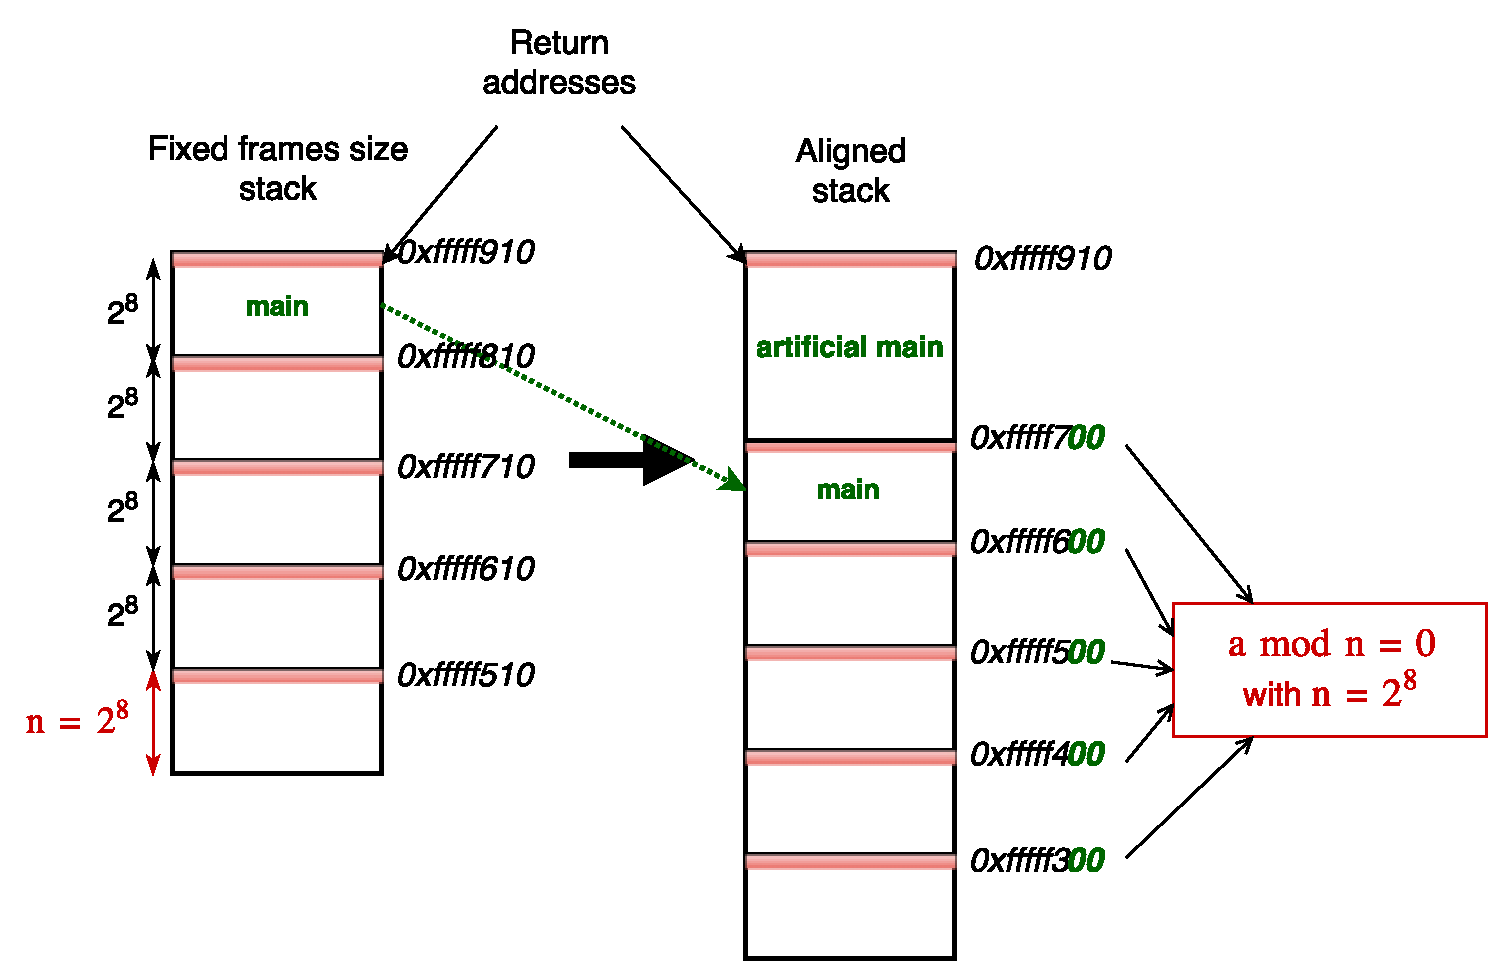
\includegraphics[scale=0.6]{images/stack_align.pdf}
\caption{Aligning CompCert stack frames}
\label{stack_align}
\end{figure}

\paragraph{Alignment algorithm.}
\label{par:Alignment algorithm}
We present in Figure~\ref{align_algo}, the algorithm used to calculate the right size in order to have the next return addresses aligned even with ASLR. The algorithm is written in pseudo assembly code.

The easiest way to understand it is to go through it with an example. On the previous examples Figure~\ref{stack_transform} and Figure~\ref{stack_align} our stack starts at the value \texttt{0xfffff910}. Hence for the continuity of the examples we keep this value. 
In Figure~\ref{stack_align} we want to have our next frame starting at the address \texttt{0xfffff700}. 
We go through the different lines of Figure~\ref{align_algo} to explain the algorithm.
\textit{next\_frame} corresponds to the value of the stack pointer which gives the starting address of the following frame.
The aim of the alignment algorithm is to verify the property $\textit{next\_frame}~mod~n=0$ for any initial value of \textit{next\_frame} given by ASLR. For the example we will take \textit{next\_frame}~=~\texttt{0xfffff840}.\\

\begin{enumerate}
	\item we copy the initial \textit{next\_frame} location into a register called \textit{reg}.\\
		  The operation is then \textit{reg}~=~\textit{next\_frame}~=~\texttt{0xfffff840}
	\item \textit{reg} = \textit{reg} \& $(n-1)$ = \texttt{0xfffff840} \& \texttt{0x000000ff} = \texttt{0x00000040}\\
		In our examples we have $n-1 = 2^8-1$ = \texttt{0x000000ff}
	\item \textit{reg} = \textit{reg} $+(n-4)$ = \texttt{0x0000040} $+$ \texttt{0x000000fc} = \texttt{0x00000140}
	\item \textit{next\_frame} $=$ \textit{next\_frame} $-$ \textit{reg} = \texttt{0xfffff840} $-$ \texttt{0x00000140} $=$ \texttt{0xfffff700}
	\item We start the function call routine, here we save registers state in the stack
	\item We store the parameters of the original \textit{main} in the stack
	\item We call the original \textit{main} function, its frame will start at the location stored in \textit{next\_frame}~$=$~\texttt{0xfffff700}
\end{enumerate}

A small remark on the example is that our algorithm only works if the last bit of the first value of \textit{next\_frame} = \texttt{0xfffff840} is \texttt{0}. However this particularity is not an issue because all compilers follow this rule since it improves the speed of execution due to alignment property.

\begin{figure}[!ht]
\centering
\begin{lstlisting}
move	reg		next_frame  
and	reg		n-1	    
add	reg		n-4    
sub 	next_frame	reg
store 	regs_state
store	parameters
call	main
	
\end{lstlisting}
\caption{Alignment algorithm}
\label{align_algo}
\end{figure}

\subsection{Detection of memory write statements}

\paragraph{Clight implementation.}
\label{par:Clight implementation}

We chose to implement the detection of dangerous statements and also the runtime checks of those statements at the Clight level.
This choice is explained by the fact that Clight is a high-level language in the compilation steps of CompCert (it is the closest to C so the syntax is really similar).
Indeed, doing our transformations at a high-level is much easier since all the complex compilation operations are done later in the process.
For example by using Clight we do not need to bother with low-level objects like registers which if misused can modify the program unexpectedly.
Furthermore Clight is a compilation step placed before any optimization of CompCert.
This means that our implementation can be optimized automatically by CompCert thus improving our performance.

\paragraph{Clight semantic.}
\label{par:Clight semantic}

We have to make sure that we cover all possibly harmful statements with our runtime protection.
Since we are working with the compiler CompCert we are going to take advantage of it.
CompCert has multiple compilation steps which have all been proven from C to assembly language.
To make these proofs, a semantic was defined for each language of the compilation. The semantics all relate to the memory model briefly described in Section~\ref{sub:sfi_comp}.
To detect all dangerous statements we looked at the semantic of Clight and found all statements that in the memory model could write freely in the memory.\\

\begin{figure}[!ht]
\centering
\begin{lstlisting}[language=Caml]
Inductive statement : Type :=
  | Sskip : statement
    (**r do nothing *)
  | Sassign : expr -> expr -> statement
    (**r assignment [lvalue = rvalue] *)
  | Sset : ident -> expr -> statement 
    (**r assignment [tempvar = rvalue] *)
  | Scall: option ident -> expr -> list expr -> statement
    (**r function call *)
  | Sbuiltin: option ident -> external_function -> typelist -> list expr -> statement
    (**r builtin invocation *)
  | Ssequence : statement -> statement -> statement 
    (**r sequence *)
  | Sifthenelse : expr  -> statement -> statement -> statement
    (**r conditional *)
  | Sloop: statement -> statement -> statement 
    (**r infinite loop *)
  | Sbreak : statement   
    (**r [break] statement *)
  | Scontinue : statement
    (**r [continue] statement *)
  | Sreturn : option expr -> statement 
    (**r [return] statement *)
  | Sswitch : expr -> labeled_statements -> statement
    (**r [switch] statement *)
  | Slabel : label -> statement -> statement
  | Sgoto : label -> statement
\end{lstlisting}
\caption{Clight statements}
\label{clight_statements}
\end{figure}

In Figure~\ref{clight_statements}, we have exposed all the Clight statements. Among them we are going to focus on the ones that change the state of the memory. When looking at the semantic given to these statements, only four of them can change the state of the memory: \textit{Sassign}, \textit{Sbuiltin}, \textit{Sreturn}.

\begin{itemize}
	\item \textbf{\textit{Sassign}}, are used to assign value to variables, it could be considered as an equivalent of ``='' in C. These statements will be targeted by our approach.
	\item \textbf{\textit{Sbuiltin}}, are used to call builtin functions, which are functions created by CompCert that will be expanded later in the compilation. These statements call functions we trust, that is why we will not consider them as dangerous. We could also look at the builtin functions and modify their code to make them safe.
	\item \textbf{\textit{Sreturn}}, these statements invoke the function call routine. They are also trusted statements, we will not need to add runtime checks on them.
	\item \textbf{\textit{Sset}}, could have been problematic. However they are only used to set value to temporary variables which means that they can't freely access the memory.
	\item The other statements are all kind of control flow statements, they do not change the memory state.
\end{itemize}

Among all the statements, our security checks will only apply to the \textit{Sassign} statements.
Furthermore we can limit ourselves to \textit{Sassign} statements whose left expression can write directly in the memory. Left expressions are the expressions explicitly on the left of the ``='' symbol, they are the only expressions which enable us to write in the memory (``Sassign left\_expr right\_expr'' $\leftrightarrow$ ``left\_expr = right\_expr''). The left expressions targeted are then mostly pointers dereference. To be sure that we have all the dangerous instructions, we reiterate the same approach and we take a look at the semantic of the left expressions in Clight.\\
After checking the semantic of the left expressions, only two types of left expressions are able to reference a location in the memory.

\begin{itemize}
	\item \textbf{\textit{Ederef}}, as we predicted these expressions dereference pointers and will be targeted by our approach.
	\item \textbf{\textit{Efield}}, they refer to fields of structure and can also point to locations in the memory. These expressions will also be secured with runtime checks.
	\item \textbf{\textit{Evar}} are the last left expressions possible. \textit{Evar} are tied down to a location in the memory. They can't reach return addresses locations hence they are not threats.
	\item The other expressions are not left expressions which means they do not write in the memory and they are not dangerous in our case. Unary operators \textit{Eunop}, binary operators \textit{Ebinop}, constants \textit{Econst\_int} \textit{Econst\_float} are examples of such expressions.
\end{itemize}

We finally have defined the profile of the dangerous statements that have to be targeted by our approach. To sum it up, the targeted statements are all the \textit{Sassign} whose left expression is either \textit{Ederef} or \textit{Efield}.

Now that we can detect the dangerous statements we will now add the runtime checks in the Clight code which will terminate our implementation.

\subsection{Securing memory write statements}
\label{sub:implem_check_address}
We want to add a protection mechanism which prevents any dangerous statement from writing on a return address location. These return addresses locations have two special traits:
\begin{enumerate}
	\item they only exist in the memory area of the stack
	\item thanks to our previous modifications, their locations $a$ verify $a~mod~n=0$
\end{enumerate}
If a statement try to write on an address with these two properties then it is an illegal execution and our mechanism will trigger an error behaviour like crashing. The Figure~\ref{runtime_check} explained earlier can be used as a reminder of the principle of these runtime checks.

\paragraph{Distinguish stack and heap addresses.}
\label{par:Distinguish stack or heap}
A program can only use the stack and the heap to store data during runtime. Since return addresses are only present in the stack we need a way to differentiate stack and heap addresses.
In x86 architecture, the stack usually grows downwards in direction of the heap. Therefore the addresses of the stack occupy the high addresses and the heap the low ones. 
The idea is to divide the memory space for the program data into two distinct part. The high addresses for the stack and the low for the heap. \\
We defined the clear separation at the address \texttt{0xff000000}. Every address bigger than \texttt{0xff000000} is considered as part of the stack. Reciprocally every address smaller is part of the heap. However this assumption is not always true, in extreme cases the stack or the heap might overflow over this limit. To ensure that our criteria becomes a truth we propose a solution in the future works section Chapter~\ref{par:guard_area}.

Figure~\ref{classic_check} presents an implementation of our runtime checks. The condition line~1 is the branch which separated addresses from the stack or the heap. Heap addresses can't be return addresses location therefore they do not continue the verification process.

\begin{figure}[!ht]
\centering
\begin{lstlisting}[language=C]
if (targeted_address > 0xff000000) {
	temp_var = targeted_address & (n-1);
	if (temp_var < 3) {
		Error behaviour
	} 
}
*targeted_address = value;
Continue execution...
\end{lstlisting}
\caption{Runtime checks}
\label{classic_check}
\end{figure}

\paragraph{Check the property $a~mod~n=0$.}
\label{par:Classic check}
The second step of the runtime check is to see if the targeted address location $a$ verifies $a~mod~n=0$. It corresponds to the code from line~2 to to line~4 of Figure~\ref{classic_check}.
\begin{itemize}
	\item At line~2 we reduce the targeted address to its $log_2(n)$ least significant bits (8 if $n=2^8)$.
Since $n$ is a power of two just comparing the least significant bits to $0$ is equivalent to checking if the address verifies $a~mod~n=0$.
For example we know that the return addresses locations of our previous example Figure~\ref{stack_align} were \texttt{0xfffff700}, \texttt{0xfffff600}, \texttt{0xfffff500}\dots
We can notice that we only need to check if the last eight bits (the last two digit in hexadecimal \texttt{00} in our example) of an address is equal to 0.
If it is we know for sure that the targeted location is a return address.\\
For a random authorized location \texttt{0xfffff7a2} and a return address location \texttt{0xfffff700} with $n=2^8$, we would have to compare \texttt{0x000000a2}(authorized) and \texttt{0x00000000}(unauthorized) with $0$. 
	\item Line~3 we actually see that we do not compare the previous calculated value with 0 but 3. The reason is that return addresses are four bytes long.
		It means that the space taken by a return address located at \texttt{0xfffff700} would be [\texttt{0xfffff700}~-~\texttt{0xffff703}]. It is logical for us to protect the whole return address space, that is why we check if the targeted address least significant bits are smaller than 3.
	\item Line~4 is executed when there is an illegal behaviour. Currently our error behaviour is to make the program crash by trying to write over some protected memory located at the address 0 which triggers a \textit{Segmentation fault}.
	\item Finally line~7 if we successfully pass the verification we are allowed to write on the dereferenced pointer \textit{temp\_var}.
\end{itemize}


Currently our protection mechanism use two \textit{if \dots then \dots else} operation in a row to protect the return addresses. The first to check if the address is in the stack and the second to check the equality $a~mod~n=0$.
Considering that we might inject our protection mechanism a considerable number of times for a program using a lot of pointer operations. We wanted to try another possible implementation that may improve the performance our runtime checks.
Hence we present in the next section an alternative to the classic \textit{if then else} called branchless statement.

\paragraph{Branchless check.}
\label{par:Branchless check}

We wanted to limit the overhead introduced by our approach by trying another way to make the protection mechanism. 

Branchless code allows one to create code with the same behaviour as a classic \textit{if then else} but without creating any branch for the processor. In other words the processor will not need to execute different code depending of the condition, the code will be linear.\\
The best way to understand it is to have an example and we show the branchless version of implementation of the protection mechanism in Figure~\ref{branchless}.

The branchless code is the code located from line~2 to line~6.
The main idea of the branchless code is to create a mask from line~2 to line~5 which will be stored in \textit{temp\_var}. If the initial value of \textit{targeted\_address} is a return address location the mask should be full of 0 so that the masking operation line~6 gives us a null pointer. In the other case the mask should be full of 1 so that the masking operation line~6 keeps the value of \textit{targeted\_address}.
The first condition line~1 is the same as before which checks if \textit{targeted\_address} is in the stack or the heap.
Branchless uses a lots of bit arithmetic and low level properties of two's complement representation of negative numbers. We are going to go through every line of branchless code with two different initial value of \textit{targeted\_address}: one is a return address location which is illegal and the other is an authorized address.


For both case we have $n=2^8$ for the chosen frames size. 
We start with an authorized address and we take the \textit{targeted\_address}~=~\texttt{0xfffff7a2}. Since we have a legal address our branchless operations should leave \textit{targeted\_address} unchanged.
\begin{enumerate}[noitemsep]
	\setcounter{enumi}{1}
	\item We want to keep the least significant bits with a \textit{and} operator (\texttt{0101} \& \texttt{1100} = \texttt{0100})\\
		\textit{temp\_var}~=~\texttt{0xfffff7a2}~\&~\texttt{0x000000ff}~=~\texttt{0x000000a2}
	\item \textit{temp\_var}~=~\texttt{0x000000a2}~-~\texttt{0x00000003}~=~\texttt{0x0000009f}
	\item A right shift bit operation (\texttt{0100} $\rightarrow$ \texttt{0010}) thirty-one times. If the value is negative then the new bits introduced on the left are equal to 1 else they are equal to 0. \\
 \textit{temp\_var}~=~\texttt{0x0000009f}~$>>$~31~=~\texttt{0x00000000}
	\item bits inversion (\texttt{0100} $\rightarrow$ \texttt{1011}) \\
		\textit{temp\_var}~=~$\sim$\texttt{0x00000000}~=~\texttt{0xffffffff}
	\item \textit{targeted\_address}~=~\texttt{0xffffffff}~\&~\texttt{0xfffff7a2}~=~\texttt{0xfffff7a2}
\end{enumerate}
The branchless operation is successful, the initial address was an authorized location, therefore \textit{targeted\_address} kept its value during the branchless and the assignment line~8 is successful.

\begin{figure}[!ht]
\centering
\begin{lstlisting}
if (targeted_address > 0xff000000) {
	temp_var = targeted_address & (n-1);
	temp_var = temp_var - 3;
	temp_var = temp_var >> 31;
	temp_var = ~temp_var;
	targeted_address = temp_var & targeted_address;
}
*targeted_address = value;
Continue execution...
\end{lstlisting}
\caption{Branchless version of the second check}
\label{branchless}
\end{figure}

We go through the case where \textit{targeted\_address} is a return address locations, we take \textit{targeted\_address} = \texttt{0xfffff700}. 
The destination is illegal, the branchless operations should leave in \textit{targeted\_address} an illegal value to make the program crash.
\begin{enumerate}[noitemsep]
	\setcounter{enumi}{1}
	\item \textit{temp\_var}~=~\texttt{0xfffff700}~\&~\texttt{0x000000ff}~=~\texttt{0x00000000}
	\item \textit{temp\_var}~=~\texttt{0x00000000}~-~\texttt{0x00000003}~=~\texttt{0xfffffffd} (signed representation)
	\item \textit{temp\_var}~=~\texttt{0xfffffffd}~$>>$~31~=~\texttt{0xffffffff}
	\item \textit{temp\_var}~=~$\sim$\texttt{0xffffffff}~=~\texttt{0x00000000}
	\item \textit{targeted\_address}~=~\texttt{0x00000000}~\&~\texttt{0xfffff7a2}~=~\texttt{0x00000000}
\end{enumerate}
The value of \textit{targeted\_address} at the end is zero. Hence the assignment line~8 will make the program crash since zero is a protected memory area. The initial address was a return address location which means that the illegal operation crashed as we wanted.

This way we can notice that we got the same result as with the \textit{if then else} check but without creating any branch. In our case it is not possible to 
replace the first \textit{if then else} condition because it would even force heap addresses to go through the second check which we do not want.
\newpage

\section{Evaluation of the implementation}
We will show first in this section that our implementation is effective. 
Afterwards we will present different benchmarks we did to measure the cost of our transformations on different criteria like speed or size of the programs.
To conclude we will discuss multiple ideas to improve the current approach.

\subsection{Evaluation of security}
For the example we are going to confront the buffer overflow presented Figure~\ref{buffer_overflow_code} with our implementation. We modified the code of the buffer overflow a little to simplify the test. To make things easier we just added the function \textit{strcpy} in the program's code instead of calling it from another library. This way the vulnerable code of \textit{strcpy} will be compiled with our transformation and be secured instead of compiling the whole external library.


To check the effectiveness of our approach we compile the buffer overflow in two different ways.
The first time we compile it with our implementation but we do not activate the protection mechanism. 
In other words this executable has fixed frames size but we did not insert the runtime checks so it is still vulnerable to the buffer overflow. 
The second executables is compiled with our whole mechanism and is protected with runtime checks.
However the two executables were compiled with the same stack frames size, $n=2^6$.
The output of the two binaries are presented Figure~\ref{output_weak}~and~\ref{output_protected}. 

\begin{figure}[!ht]
\textcolor{gray}{terminal\$~} ./buff\_comp\_weak \$(python -c 'print "a"*44+"\textbackslash{xb0}\textbackslash{x84}\textbackslash{x04}\textbackslash{x08}"')\\
Address of evil\_code = 0x080484b0 \\

Stack before:\\
0xf756e724   \\
0xff9dab44   \\
0xff9dac74   \\
0x00000002   \\
0xf7731000   \\
\dots\\
0xf75b2d00   \\
             \\
Stack after :\\
0xff9db132   \\
0xff9dab44   \\
0xff9dac74   \\
0x61616161   \\
0x61616161   \\
\dots   \\
0x61616161   \\

Argh, we got hacked!\\
Segmentation fault (core dumped)
\caption{Output from vulnerable CompCert executable}
\label{output_weak}
\end{figure}


\paragraph{Fixed stack frames without protection (Figure~\ref{output_weak}).}
\label{par:Fixed stack frames without protection.}

Like in Figure~\ref{output_buffer} we can see that we have printed \textit{Argh, we got hacked!} which means we managed to execute the function \textit{evil\_code}. The buffer overflow is successful, we can see that we needed to change the input for the attack to work. Indeed since we changed the compiler and the stack layout the input had to be different to manage the attack. 

\begin{figure}[!ht]
\textcolor{gray}{terminal\$~} ./buff\_comp\_weak \$(python -c 'print "a"*44+"\textbackslash{xc0}\textbackslash{x85}\textbackslash{x04}\textbackslash{x08}"')\\
Address of evil\_code = 0x080485c0\\

Stack before:       \\
0xf7554724          \\
0xff9a88c4          \\
0xff9a8a04          \\
0x00000002          \\
0xf7717000          \\
0000000000          \\
0xf7598d26          \\
0xf7717d60          \\
0x08048654          \\
0xff9a88cc          \\
0xf7598d00          \\
                    \\
Address: 0xffa2b0c0 \\
Segmentation fault (core dumped)
\caption{Output from protected CompCert executable}
\label{output_protected}
\end{figure}

\paragraph{Complete implementation with protection (Figure~\ref{output_protected}).}
\label{par:Complete implementation with protection}

For the sake of the example, we enriched the error behaviour statement which now calls  ``\textit{printf(Address:~\%p,~tmp)}'' before crashing. In \textit{tmp} we stored the value of the address for which the protection mechanism triggered the error behaviour.
First of all we can see that we made the program crashed before \textit{evil\_code} was executed. Our implementation successfully does what we aimed for, we made the program crash on a dangerous program.
Furthermore we can even see the address on which the program tried to write and was not allowed to. In this example our protection mechanism crashed when the program tried to write on the address $a=\texttt{0xffa2b0c0}$. 
Since the frames size is $n=2^6$ all our return addresses location should have their least six significant bits equal to 0.
We check that $a=\texttt{0xffa2b0c0}$ is effectively a return address. First of all $a>\texttt{0xff000000}$ which means that $a$ is actually part of the stack. Moreover we need to verify the equality $a~mod~n=0 \leftrightarrow (\texttt{0xffa2b0c0})~mod~(\texttt{0x00000040}) = 0$ which is true. 
Both the conditions are fulfilled which means that $a$ is a return address location and that our mechanism properly worked.


\subsection{Evaluation of performance}

As mentioned earlier, we also want to measure the impacts that our transformation may bring in terms of memory and efficiency.
We made some experimentations in order to figure out these questions.
Furthermore we also had to verify which implementation was the most efficient between the branchless and the classic \textit{if then else}.
For our different experimentations we had 74 different C programs which were present within the CompCert project for testing purposes.
The performances of our approach are compared with the original CompCert project whose performances are similar to \texttt{gcc -O1}~\cite{Leroy:2009:FVR:1538788.1538814}.
The machine used for the benchmarks possesses four 64 bits processors Intel Xeon E5 with a capacity of 2.80GHz and 8GB of memory. The operating system of the machine is Fedora 23.
For all our executables compiled with fixed frames size we chose the smallest size possible for the programs to be able to run correctly. Our script just try to compile every program with an incrementing frames size until it manages to complete the compilation process.


\subsubsection{Efficiency}
\label{ssub:Efficiency}

We wanted to measure the efficiency of our different transformations and compare them to the original CompCert. During our test we measured four different implementations: the original CompCert, our transformation just with fixed frames size, with fixed frame size and classic \textit{if then else} runtime checks and the branchless version.
To calculate the execution time we used the Unix utility \textit{time}.
The results are presented in the following graph Figure~\ref{time_percentage_graph}.
For more relevant results we removed from all the tested programs the ones whose execution time was too short because the Unix utility \textit{time} imprecision could impact the result greatly.

\begin{figure}[!ht]
\centering
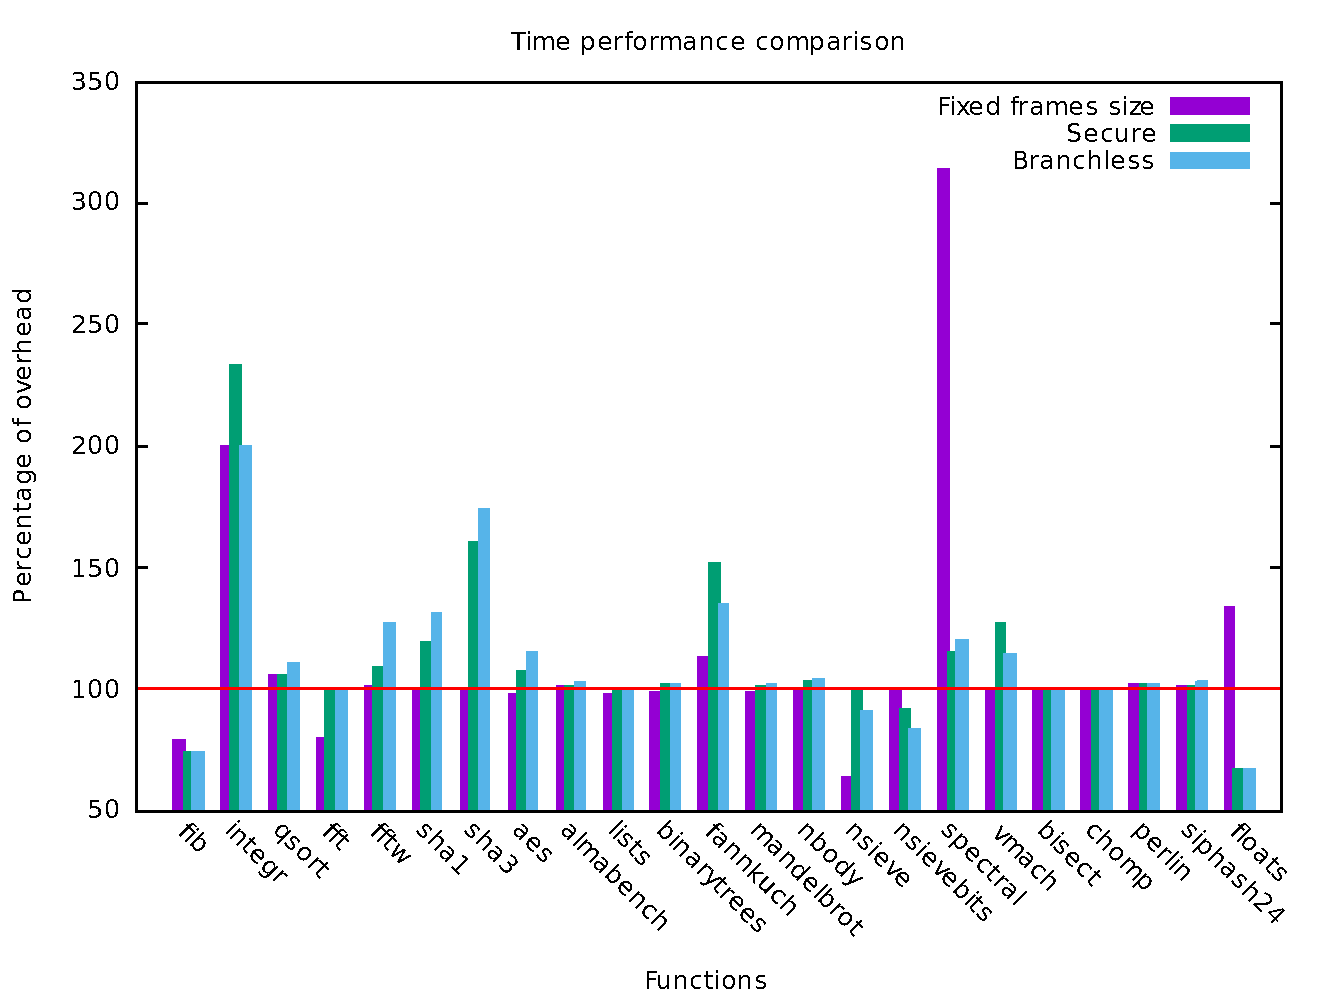
\includegraphics[width=1\textwidth]{images/time_percentage_graph.pdf}
\caption{Execution time percentages compared to the original CompCert}
\label{time_percentage_graph}
\end{figure}

We notice that the fixed size frames without protection has usually the same execution time than the original CompCert. 
We deduce that only the protection mechanism introduces overhead during the runtime.
Only in the programs \textit{spectral} and \textit{floats} we had a strange overhead which were clearly superior to the protected versions. 
Since the fixed frames size version is only a reduced version of the protected ones it seems very strange. We suspect that this overhead is due to some kind of misalignment of the addresses, more investigations would be needed to determine the exact reason of this phenomenon.

As for the comparison between the \textit{if then else} and the branchless implementations we were disappointed by the results displayed by the branchless version. Indeed the branchless is slower than the classic \textit{if then else} for most programs. \\
Actually what can makes branching instructions expensive in term of time is due to instructions pipelining. 
The modern processors usually put in their pipelines a dozen of instructions ahead of the executed one. 
The issue with branch like \textit{if then else} is that the processors try to make a prediction on the branch that is going to be executed and start pipelining the predicted branch.
If the prediction is right everything is fine, however if the prediction is wrong the whole pipeline might need to be flushed to execute the program correctly. This pipeline flush slows down the execution greatly which is why \textit{if then else} are considered slow instructions.
However in our implementations these predictions are certainly correct most of the time which would explain that the branching introduces less overhead than the branchless version.

Overall, our implementations are quite slow and some of our test programs even present up to 230\% overhead for the classic \textit{if then else} version. Even if the average is comprised between 100\% and 150\% this is still high. Nevertheless there are still ways to improve our implementations that we will present Section~\ref{par:improvement}.


\subsubsection{Relation between runtime checks and delay}

The previous test shows that the implementation which added runtime checks are slower than the one with fixed frames size without protection. We suspect that the number of runtime checks is related to the amount of delay introduced by our transformation. To verify this hypothesis we first calculated the number of runtime checks that was executed by each implementation.
We also separated the runtime checks for addresses of the stack and the heap. Indeed in our implementations addresses from the heap only need to go through one conditional jump whereas for the stack we also check the equality $a~mod~n=0$.
Figure~\ref{occurence_graph} presents the number of time our runtime checks are executed. We selected the results of the programs which had a significant amount of runtime checks. 
Most of the programs which have not been represented had no runtime checks added because they did not contain any dangerous instructions.
The number of occurrences are on a logarithm axis since the values had big gaps between them.

\begin{figure}[!ht]
\centering
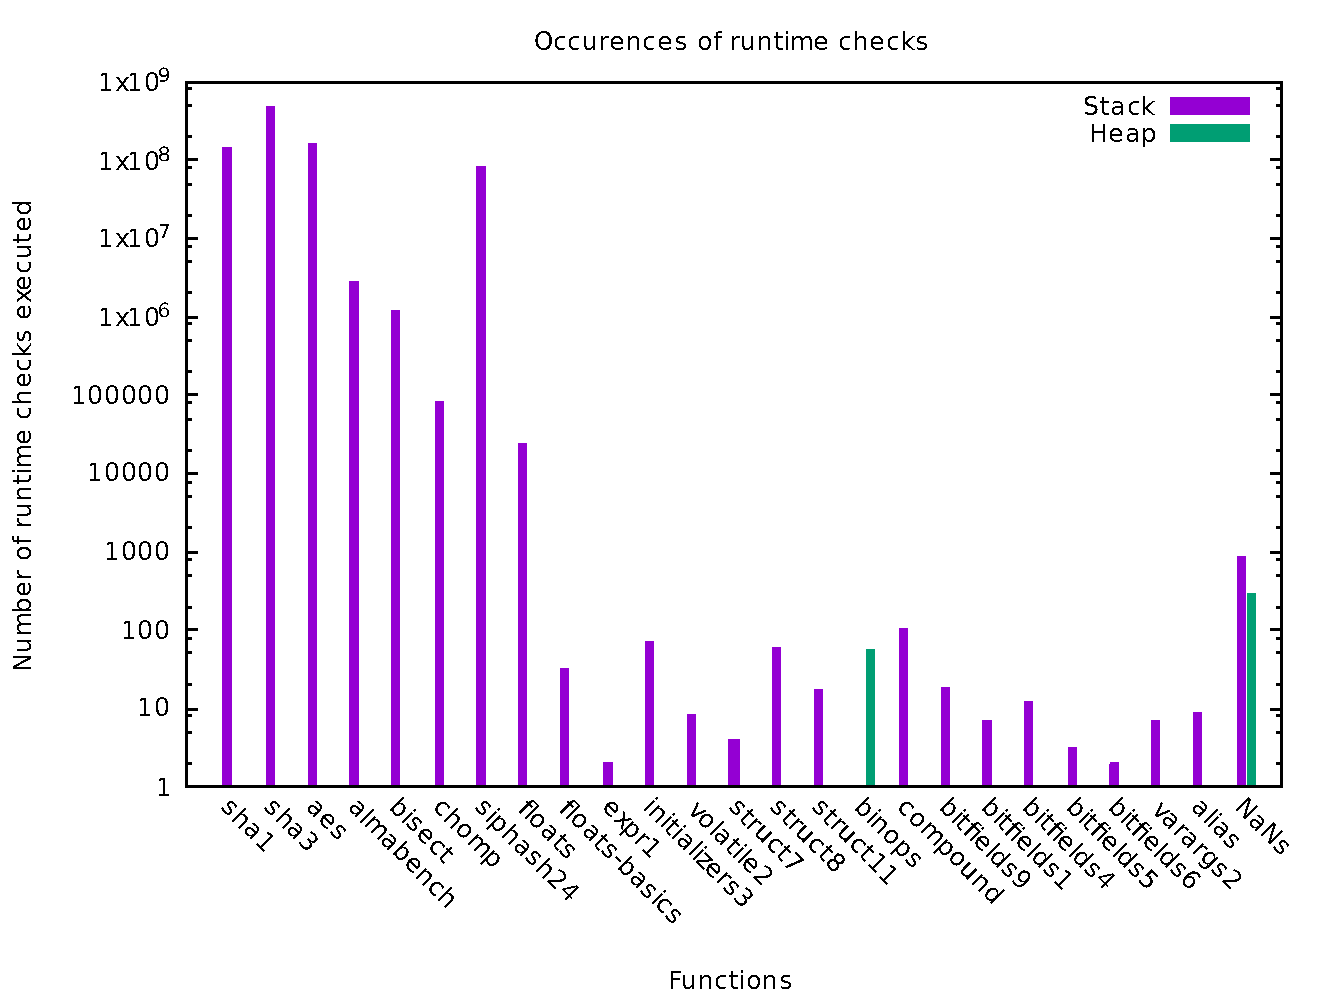
\includegraphics[width=1\textwidth]{images/occurence_graph.pdf}
\caption{Number of runtime checks executed per program}
\label{occurence_graph}
\end{figure}

First of all most of the programs write in the stack, only two of them write in the heap and most of them do not execute any dangerous instructions. Also some of the programs that had overheads in the previous figures also executes a lot runtime checks.
Especially we can notice that the program which had the most overhead \textit{sha3} compared to the version without protection is also the one which executed the biggest number of runtime checks $4,5*10^8$. \\
Following this observation we wanted to correlate the overhead introduced with the number of runtime checks executed.
We drew another graph Figure~\ref{correlation_graph} representing the percentage of delay introduced in each program depending of the number of runtime checks added. Like before the number of runtime checks axis uses a logarithmic scale to include all obtained values.

\begin{figure}[!ht]
\centering
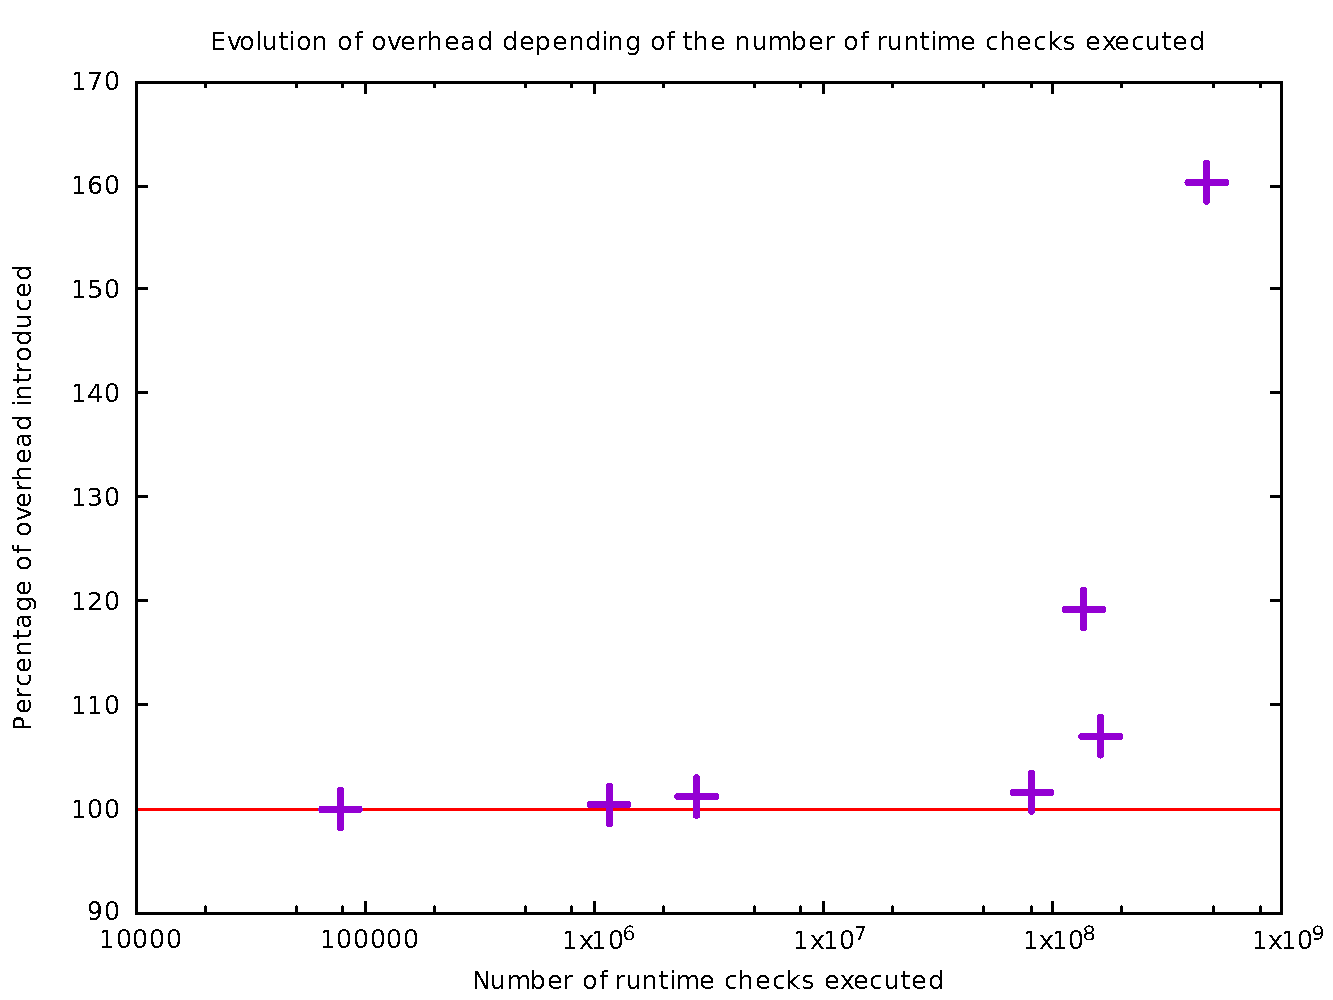
\includegraphics[width=1\textwidth]{images/correlation_graph.pdf}
\caption{Evolution of the overhead percentage depending of the number of runtime checks executed}
\label{correlation_graph}
\end{figure}
For this graph we selected only programs that had a significant amount of execution time so the percentage of overhead calculated is not too biased due to the precision of our tool (\textit{time} Unix utility). 
Furthermore among these programs we only selected the one which had executed some runtime checks during their runtime. 
After the selection we were only left with seven programs to make a graph, the results are presented Figure~\ref{correlation_graph}.

We effectively see the percentage of overhead increasing with the number of runtime checks executed.
Despite of the low number of measures, Figure~\ref{correlation_graph} presents the expected characteristic and confirm our hypothesis that the runtime checks impact the most the execution time of the programs.


\subsubsection{Stack frames size}
\label{ssub:Stack frames size}

Another figure we thought would be interesting was to see the distribution of the minimal frames size necessary for the programs to run. These data are represented Figure~\ref{frame_size_graph}.

\begin{figure}[!ht]
\centering
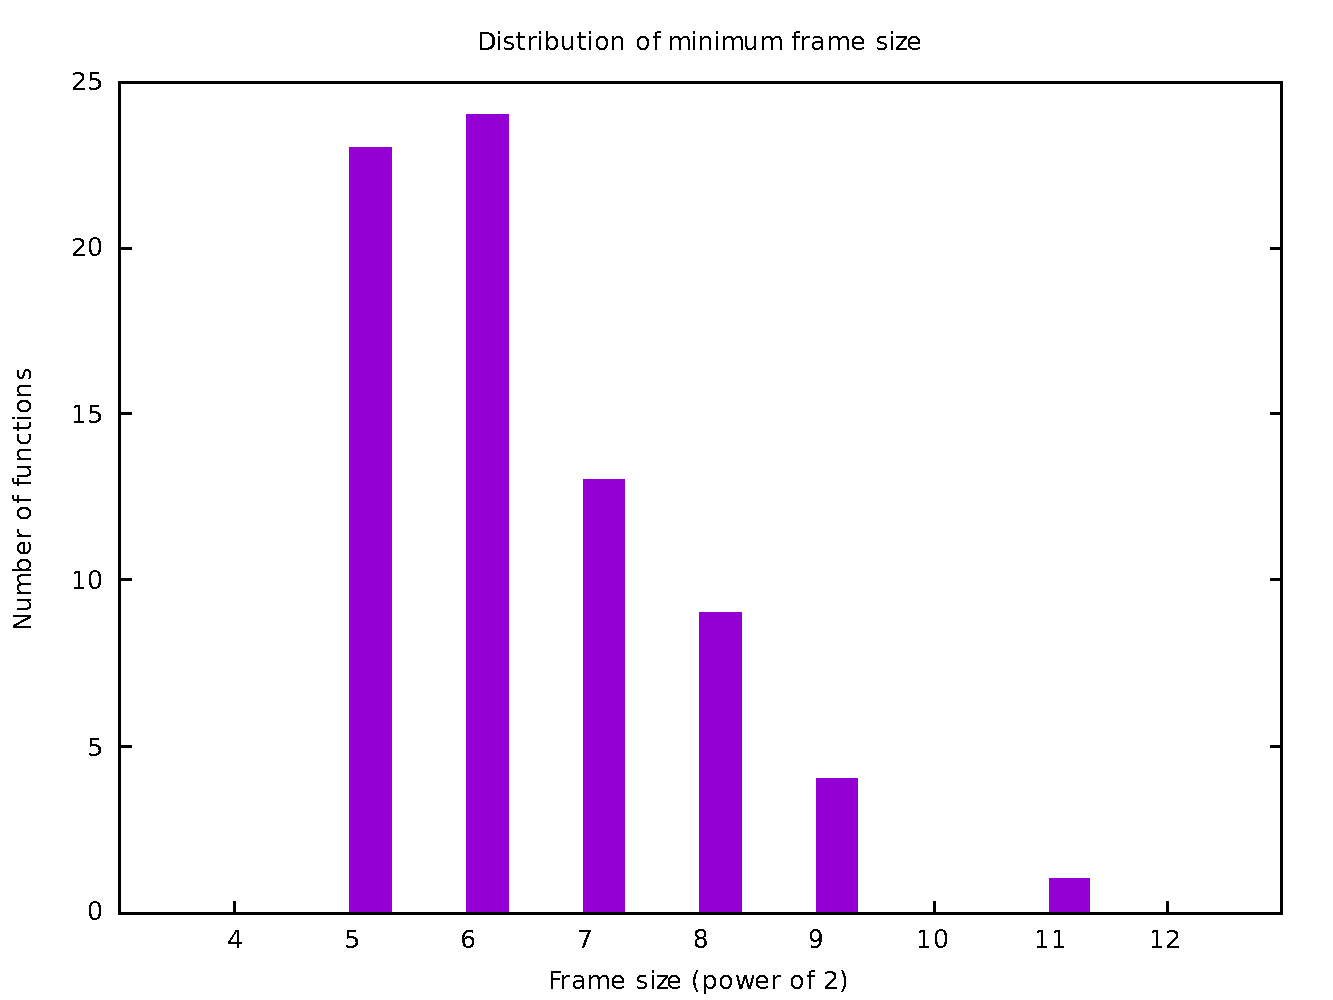
\includegraphics[width=1\textwidth]{images/frame_size_graph.pdf}
\caption{Distribution of the minimum frames size among 74 test programs}
\label{frame_size_graph}
\end{figure}

This gives us an idea about the size of the stack in the protected implementations. The results obtained show the minimal frames size required for our programs are small enough to not impact the memory usage. However the test programs we used were all relatively small and the distribution of bigger programs could be different.
A more interesting graph related to memory consumption would be the comparison of the stack maximum growth between our implementations and the original CompCert. 
%Unfortunately we did not find the time for this experimentation during the span of the internship and we hope to do it during the remaining month.

\subsection{Discussion}

In this section we are going to talk about some points that our implementation is still lacking and also ways to improve our implementation that we could explore in the future.

\paragraph{More tests.}
\label{par:More tests}
Our implementation protect return addresses by modifying the stack layout of the programs. With this guarantee we are confident that we can prevent any kind of ROP attacks. 
However we only tested our implementation with simple buffer overflows, to show that our approach is correct it would be interesting to pit our protection mechanisms against more complicated ROP attacks. Otherwise we used CompCert so that eventually we will prove the security properties of our approach . This would be an even more convincing way to affirm the benefits of our approach.

%Another test that is lacking was mentioned before. To have an idea of the impacts of our implementation of the memory consumption it would be interesting to compare the stack growth of a normal program with one compiled with our modified CompCert compiler.
\paragraph{Guard area between the stack and the heap}
\label{par:guard_area}
To ensure that either the stack or the heap grows too much and exceeds their designed area we want to put a guard area in the memory. The idea is to define a specific area in the memory, for example [\texttt{0xee000000 - \texttt{0xff000000}}], where it is forbidden to write. If an instruction writes illegally in the guard area the program will detect it and will crash.\\
The principle is represented in Figure~\ref{guard}. Indeed we can see that the stack and the heap are clearly separated by the guard area located between [\texttt{0xee000000 - \texttt{0xff000000}}]. Thus we are sure that every address above \texttt{0xff000000} are part of the stack.

\begin{figure}[!ht]
\centering
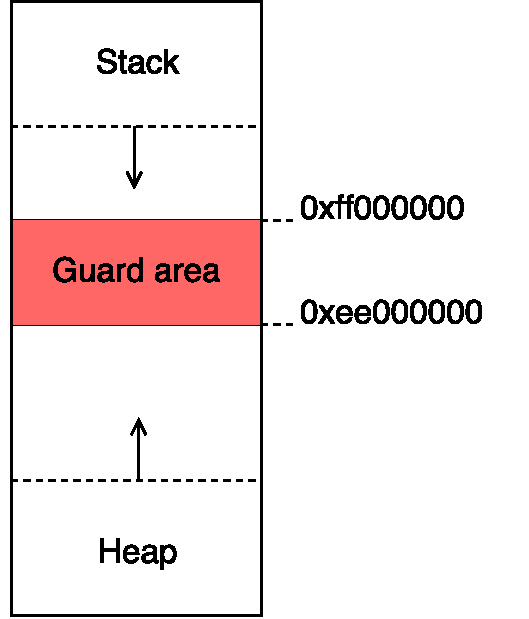
\includegraphics[scale=0.6]{images/guard.pdf}
\caption{Guard area for the memory}
\label{guard}
\end{figure}

To detect the write in the guard one possible way is to initialize the area with 0 for example. If we detect a bit in the guard area with the value 1 then we know that the guard has been corrupted and we make the program crash. Since our approach protects against ROP attacks, which takes effect when returning from a function, it is adequate to check the integrity of the guard area at the end of each function before returning.
To be honest the guard area has not been implemented yet. Most of the programs do not have a stack or a heap which grows enough to exceed the limit of \texttt{0xff000000} so we were able to do satisfactory tests nevertheless. This guard area is necessary for our implementation to be complete and we hope that we will be able to do it during the remaining time of the internship.

\paragraph{Protection of runtime checks.}
\label{par:Protection of runtime checks}
Actually in our implementation we protect return addresses with runtime checks but we never protect these runtime checks. As in SFI we also need to prevent malicious instructions to avoid going through these checks. Therefore we need to make sure that is not possible for a program to freely jump in the code. This way an attacker would be able to bypass the security measures we established.
In the C language the only expression that could allow such operations would be function pointers. Function pointers allow one to execute the code addressed by the pointer.
The simplest solution would be to totally forbid the usage of function pointers which would solve our issue.
We could also adapt ideas of SFI~\cite{Mccamant_evaluatingsfi} like creating memory chunks and aligning them in order to render the runtime checks atomic. This idea is similar to our approach, it would need to transform the structure on the memory for the code and then perform runtime checks to make sure we only jump to authorized locations.

\paragraph{Ways of improvement.}
\label{par:improvement}
We saw in the earlier section that our implementation was relatively slow compared to the original CompCert. Furthermore the amount of overhead was dependent of the number of runtime checks executed.
The idea would be to reduce the number of runtime checks effectively done.
We can certainly narrow down the number of dangerous statements detected. For example Figure~\ref{harmless} presents some harmless C code that would be protected by our approach but does not present any vulnerability for a ROP attack. The pointer presented here points to an address of the heap so if the heap does not overflow on the stack it's not possible for the pointer \textit{bar} to write on a return address as it is.
We can see clearly that the protection mechanism that will be introduced in this code is not necessary and will just slow down the program.
To detect these kind of occurrences, it would be necessary to make a static analysis of the code and pinpoint the statements that present a vulnerability for ROP attacks.
If we could implement such static analyser \textcolor{green}{find ref maybe} the overhead from our implementation will be greatly reduced since we know the more we add runtime checks the more our program will slow down.

\begin{figure}[!ht]
\begin{lstlisting}
void foo(){
	int *bar = malloc(sizeof(int));
	*bar = 1;
}
\end{lstlisting}
\centering
\caption{Example of harmless C code }
\label{harmless}
\end{figure}

\paragraph{Transparency.}
\label{par:Transparency}
Our approach should leave safe programs behaviour unchanged. We do not want our implementation to change harmless programs in any way. Our runtime checks are transparent since the error behaviour is only triggered during illegal executions, otherwise the code executed will stay the same. The other modifications were done at the stack level, the stack does not exist at the level of the C language.
Hence apart from inline assembly (that we want to forbid) it should not be possible to interact with the stack with C. The only way left would be a program which uses direct addressing, in other words a C program which gives raw addresses to pointers like the statement \texttt{pointer = 0xff000022}.
Such program is considered unsafe anyway and with the existence of ASLR the behaviour of the program would be unpredictable.

For these reasons we are confident that our implementation is transparent, but a stronger guarantee would be to give a proof of transparency.

\newpage
\section{Conclusion}
\label{sec:Conclusion}
We presented in this paper a security techniques called Software Fault Isolation which uses software methods to isolate the execution of dangerous modules. Hence SFI enables protected program to use external modules without taking the risk of compromising its execution. SFI has the benefits of demonstrating good performances in term of speed compared to other memory protection approach and also has a relatively small TCB. In this report we presented various implementations of SFI and especially the last one which used the certified compiler CompCert~\cite{Kroll:2014:PSF:2708449.2708686}. \\
Even though SFI has many strong points it can be considered lacking when it comes to securing the return addresses. Indeed few solutions were explained to face this issue and those were usually not easily adaptable or brought a lot of overheads. More importantly one the most important category of cyber attacks called ROP attacks explicitly target these return addresses to modify the flow control of the programs in their favour.

Therefore we propose a solution which is reliable and relatively efficient to protect return addresses from being corrupted. Our idea is to modify the structure of the stack in order to have an easy way to know the locations of all the return addresses. Afterwards we add runtime checks before the instructions that can compromise the integrity of the return addresses. These runtime checks take advantage of the new stack layout to forbid any illicit write on the return addresses locations.

We did an implementation of our approach with the compiler CompCert for the x86-32 architecture. Even though the implementation is not totally completed, the main work has been carried out and it successfully blocked programs containing simple buffer overflows. The different experimentations show that our transformations diminish the efficiency of our compiled modules proportionally to the number of runtime checks. We estimate that each runtime checks adds an average overhead of \textcolor{green}{number}. Thus the diminution of the efficiency varies greatly depending of the number of dangerous instructions that has to be tested in the compiled code.

However our implementation still has ways of improvement by optimizing the runtime checks efficiency or by reducing the number of runtime checks added. For example, by using static analysis we could refine our detection of dangerous instructions and narrow down the previous selection which could improve our performances greatly.


\newpage
\bibliography{ref}
\bibliographystyle{plain}
\end{document}
%%% Local Variables:
%%% mode: latex
%%% TeX-master:
%%% End:

